\documentclass[]{spie}  %>>> use for US letter paper
%%\documentclass[a4paper]{spie}  %>>> use this instead for A4 paper
%%\documentclass[nocompress]{spie}  %>>> to avoid compression of citations
%% \addtolength{\voffset}{9mm}   %>>> moves text field down
%% \renewcommand{\baselinestretch}{1.65}   %>>> 1.65 for double spacing, 1.25 for 1.5 spacing 

\usepackage[]{graphicx}
\usepackage{caption}
\usepackage{subcaption}
\usepackage{xcolor}
\usepackage{listings}
\usepackage{hyperref}
\def\arcsec{$^{\prime\prime}$}

\title{The LSST Metrics Analysis Framework (MAF)} 

\author{R. Lynne Jones\supit{a}, Peter Yoachim\supit{a}, Srinivasan
  Chandrasekharan\supit{b}, Andrew J. Connolly\supit{a}, Kem
  H. Cook\supit{c}, {\v Z}eljko Ivezi{\'c}\supit{a},  K. Simon Krughoff\supit{a}, Catherine Petry\supit{d}, Stephen T. Ridgway\supit{b}.
\skiplinehalf
\supit{a}University of Washington, Physics-Astronomy Bldg., 3910 15th
Ave NE,  Seattle, WA, USA; \\
\supit{b}National Optical Astronomy Observatory, 950 N Cherry Ave, Tucson,
USA\\
\supit{c}Eureka Scientific, Inc., 220 Duxbury CT, San Ramon, CA, USA\\
\supit{d}University of Arizona, 933 N Cherry Ave, Tucson, AZ, USA\\
}

\authorinfo{Further author information: (Send correspondence to R.L. Jones)\\R.L.  Jones.: E-mail: ljones@astro.washington.edu, Telephone: 1-206-543-9487}

%>>>> uncomment following for page numbers
% \pagestyle{plain}    
 
  \begin{document} 

  \maketitle 

\lstset{
language=Python,
basicstyle=\ttfamily\scriptsize,
breaklines=true,
tabsize=4,
commentstyle=\ttfamily\color{red}\it,
keywordstyle=\ttfamily\color{blue!90!black}\bf,
keywords=[2]{True,False, self},
keywordstyle={[2]\ttfamily\color{yellow!80!black}},
%emph={Metric,__init__, run},          
%emphstyle=\ttfamily\color{red!80!black},    
%identifierstyle=\color{blue},
stringstyle=\color{green!70!black},
showstringspaces=false
}


%%%%%%%%%%%%%%%%%%%%%%%%%%%%%%%%%%%%%%%%%%%%%%%%%%%%%%%%%%%%% 
\begin{abstract}
We describe the Metrics Analysis Framework (MAF), an open-source
python framework developed to provide a user-friendly, customizable,
easily-extensible set of tools for analyzing data sets. MAF is part of
the Large Synoptic Survey Telescope (LSST) Simulations effort. Its
initial goal is to provide a tool to evaluate LSST Operations
Simulation (OpSim) simulated surveys to help understand the effects of
telescope scheduling on survey performance, however MAF can be applied
to a much wider range of datasets. The building blocks of the
framework are {\tt Metrics} (algorithms to analyze a given quantity of data),
{\tt Slicers}
(subdividing the overall data set into smaller data slices as relevant
for each {\tt Metric}), and {\tt Database} classes (to access the dataset and read
data into memory). We describe how these building blocks work
together, and provide an example of using MAF to evaluate different
dithering strategies. We also outline how users can write their own
custom {\tt Metrics} and use these within the framework. 
\end{abstract}

\keywords{Large Synoptic Survey Telescope, LSST, Metrics Analysis
  Framework, MAF, Operations Simulation, OpSim, simulation, metrics}

%%%%%%%%%%%%%%%%%%%%%%%%%%%%%%%%%%%%%%%%%%%%%%%%%%%%%%%%%%%%%
\section{INTRODUCTION}
\label{sec:intro}  

As LSST moves toward construction, significant effort is being
invested in understanding the effect of telescope scheduling on the
overall performance of the survey. The LSST Operations Simulations
group is working toward this goal by producing simulated
surveys created with a range of observing strategies. These simulated
surveys are created by the Operations Simulator (OpSim)\cite{opsim3,
  opsim2, opsim1}. Each survey includes a detailed model of the
telescope pointing and movement capability, weather conditions,
scheduled and unscheduled downtime, and a scheduler algorithm which
can be programmed with different sets of requested observations. The
output of each simulated survey run is a simulated pointing
history for LSST, consisting of approximately 2.5 million visits for a
full 10-year simulation. LSST
plans currently call for each visit to consist of two 15-second
back-to-back exposures.  The OpSim output includes the sky coordinates
and filter used for these visits, together with the observing conditions (airmass, seeing,
sky brightness, limiting magnitude, etc.) of each visit, along with
records of the telescope state over the 10-year simulation and
information relevant to the internal state of the simulator itself. To
help evaluate these simulated survey outputs, we have built the LSST
Metrics Analysis Framework (MAF).

In broad overview, MAF is an open-source python software framework that
provides a user-friendly, easily-extensible, easily-customizable set of tools to 
\begin{itemize}
\item{read the OpSim simulated survey data from a database,}
\item{slice the data according to the values of single or multiple
columns within the data or the spatial location of the data points,}
\item{apply various algorithms (metrics) to each data slice, saving the results,}
\item{and visualize the metric results,}
\end{itemize}
while also preserving metadata about the source of the data and how the
data was sliced. For visualization, MAF can automatically generate reasonable plot labels and titles, but
the user maintains the ability to override these defaults and provide custom
labels, titles, axes ranges, etc. Additional utilities make it easy to
add new data columns `on the fly' for run-time extension of
existing database tables. More details on the overall design are
described in Section~\ref{sec:fwdesign}. 

An example of analyzing an OpSim simulated survey using MAF is
described in Section~\ref{sec:examples}, including a brief comparison
of how a user can evaluate different potential dithering methods.

MAF is intended to be extensible, allowing
users to easily write their own algorithms for metrics, which can then be
plugged into the framework and used in the same manner as any of the
provided metrics. Users can also write new data slicing classes if
needed, as well as point the framework to any kind of database. Base
classes demonstrate the APIs for each of these aspects of the
framework, and documentation (including tutorials) is provided online
at
{\url
{http://ls.st/ziz}}\footnote{Throughout the text, shortened URL
  have been used. Please see
  Appendix~\ref{app:urls} for the full URL} .  While the primary goal of
MAF is to analyze the LSST OpSim outputs, we have built the framework
to be easily applicable to more general use-cases as well. 

We anticipate that the most common extension of MAF will be users
writing their own metric algorithms ({\tt Metrics}), specifically to address their science
concerns. A demonstration of the {\tt Metric} API with a view towards the
requirements when writing new {\tt Metrics} is provided in Section~\ref{sec:MetricAPI}.

All code for LSST MAF can be git cloned from, or browsed online at, the LSST Stash 
repository, {\url{http://ls.st/pxj}}. 


\section{Framework Design}
\label{sec:fwdesign}

\begin{figure}
\centering
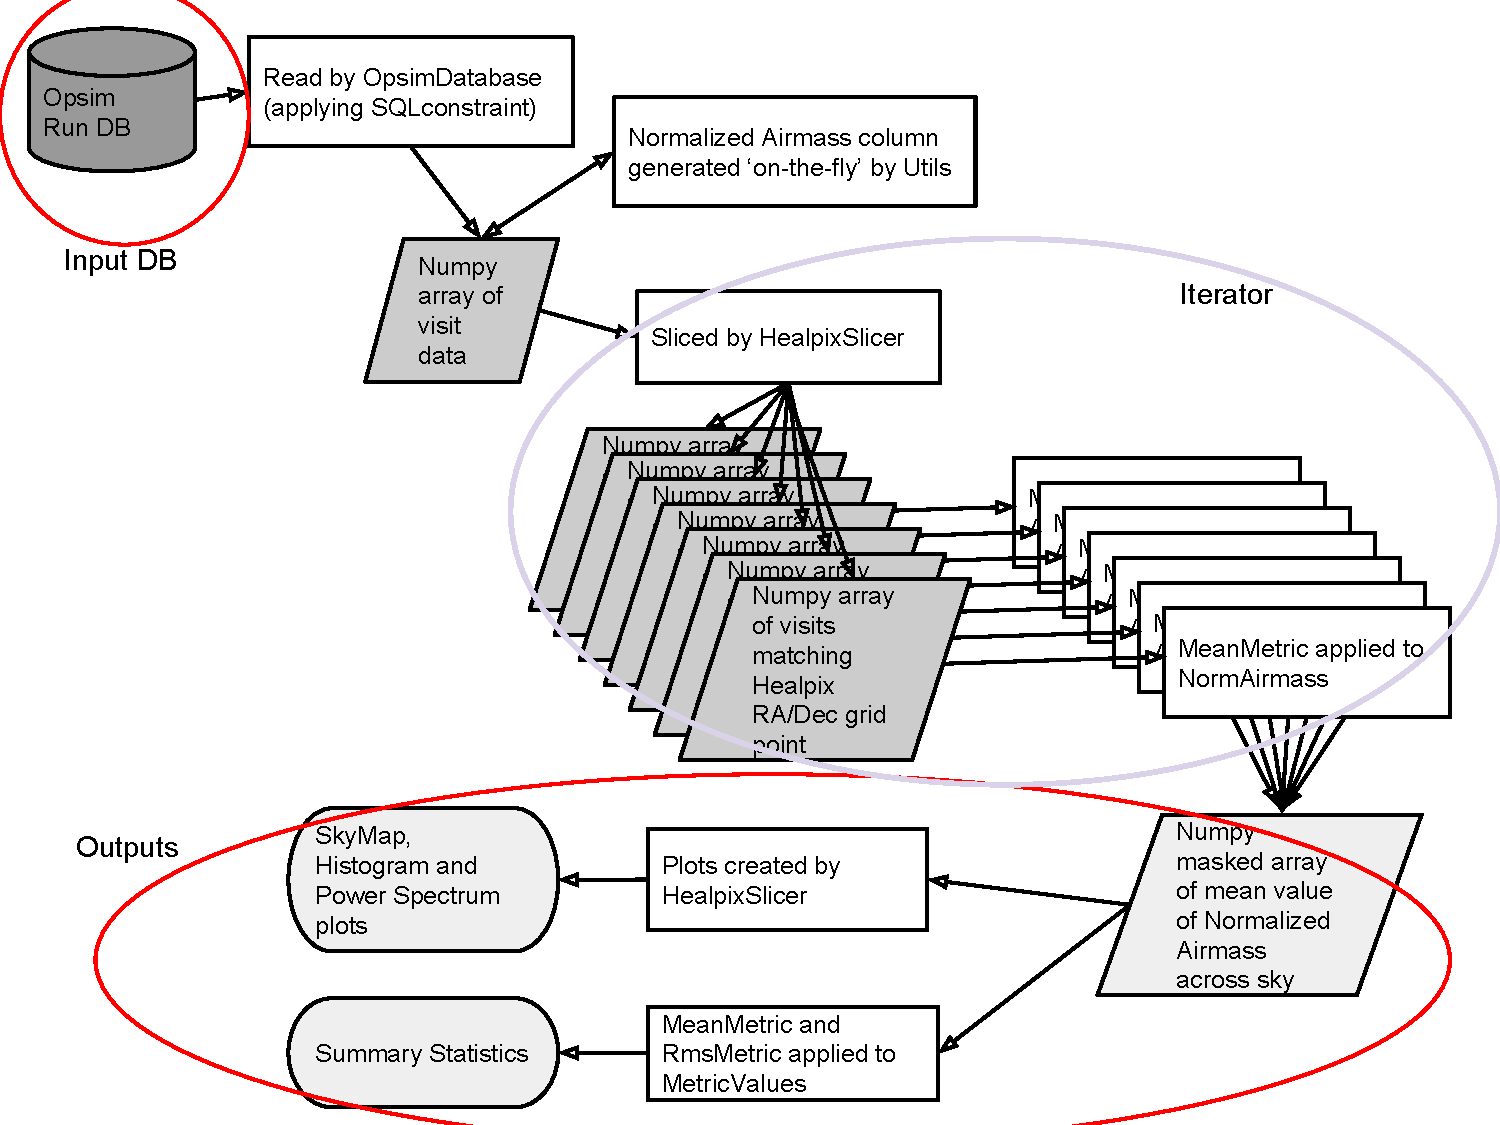
\includegraphics[height=9cm]{figures/maf_flowchart}
\caption[]
{ \label{fig:flowchart}
An illustration of the flow through MAF and interaction of MAF
objects. For this illustration, we have chosen the use-case of
calculating the mean value of the `normalized airmass' across the
sky. The normalized airmass is the airmass of each visit divided by
the minimum airmass that the field would achieve, if it was observed
on the meridian. The normalized airmass is not one of the columns
provided by the OpSim database, so we calculate this for each visit
using the MAF utility to add columns `on the fly' and merge it into
the numpy array describing the properties of each visit. Because we
want to calculate the mean value of the normalized airmass at each
RA/Dec value across the sky, we use a {\tt HealpixSlicer} to determine
the visits which overlap each Healpixel RA/Dec grid point - these are
the `data slices' passed to the {\tt MeanMetric}. The {\tt MeanMetric}
is configured to operate on the `normalized airmass' column, and
returns the mean value of this column in each data slice, as the
slicer iterates through all data slices. The values at each Healpixel
are combined to generate the mean values of the normalized airmass
across the sky. This metric data is saved to disk and used to generate
visualizations of the metric data by the {\tt HealpixSlicer}: a sky
map, a histogram and a power spectrum plot (the types of
visualizations are slicer-dependent). Summary statistics, such as the
mean of all metric data values across the sky and the RMS of these
values, can also be calculated. }
\end{figure}

The heart of the MAF framework are the {\tt Metrics} and {\tt Slicers}. These
basic classes correspond to defining ``what algorithm is being
calculated with the data'' (the {\tt Metric}) and ``what subset of data is being
evaluated'' (the {\tt Slicer}). As some examples: if we want to
analyze ``the mean airmass of all visits'', the {\tt Slicer} would simply
pass all visits to a {\tt Metric} which calculates the mean of the airmass
values; if we want to analyze ``the mean airmass as a function of
RA/Dec'', the {\tt Slicer} would identify visits which overlap a series of
RA/Dec points and pass each of those subsets to a {\tt Metric} which
calculates the mean of those airmass values. In these two examples,
the {\tt Slicers} (defining the subset of data being evaluated at once) are
different, but the {\tt Metric} itself (what calculation is being done) is
the same. Some more examples: if we want to analyze ``the mean single
visit limiting magnitude as a function of RA/Dec'' as well as ``the
total number of visits as a function of RA/Dec'', we would use the
same {\tt Slicer} but different {\tt Metrics}. These examples emphasize a
fundamental point about the framework: {\tt Metrics} and {\tt Slicers} have been
built to be modular and interchangeable.

These modules, and other modules of MAF, are described in this
section. 

\subsection{The {\tt Metrics} module}

{\tt Metrics} are simply
algorithms to analyze a given quantity of data. MAF provides a set of
{\tt Metrics}
that include a number of very simple algorithms, as well as some more
complex {\tt Metrics} focused on analyzing various aspects of the cadence of
observations or the technical performance of an OpSim run. The simple
{\tt Metrics} include {\tt MeanMetric}, {\tt MinMetric}, {\tt
  MaxMetric}, {\tt MedianMetric}, {\tt RmsMetric}, {\tt
  RobustRmsMetric}, {\tt FullRangeMetric}, {\tt BinaryMetric},
{\tt PercentileMetric}, {\tt FracAboveMetric}, {\tt FracBelowMetric},
{\tt SumMetric}, and {\tt CountMetric}. These can be applied to any column in the data,
making these {\tt Metrics} themselves flexible and easily reusable pieces of
code. A few of the more complex metrics include the {\tt CoaddM5Metric} to
calculate the coadded depth of a set of visits, {\tt
  ProperMotionMetric} and {\tt ParallaxMetric} to analyze the expected
precision of proper motion and parallax measurements for a given OpSim
simulation, the {\tt UniformityMetric} to analyze the difference between a
given distribution of visits and a uniform distribution (using a K-S
test), and {\tt VisitGroupsMetric} to analyze how groups of visits are
distributed. A full list of included {\tt Metrics} is provided in the MAF
documentation, although we anticipate that users will wish to write
new {\tt Metrics} specific to their science.

\subsection{The {\tt Slicers} module}

The {\tt Slicers} subdivide the larger OpSim output data into well-defined subsamples, such as `all
visits', `all visits overlapping a particular
Healpixel\footnote{Healpixels refer to the HEALpix (Hierarchical Equal
  Area isoLatitude Pixelisation) tessselation of the
  sphere\cite{healpix}}, RA/Dec grid
point', `all visits to a particular OpSim FieldID', or `all visits
with a particular data value within a given interval (of airmass, seeing, night, or any other
column in the data)'. We can iterate through all of these subdivisions
using methods defined in the {\tt Slicer}, thus iterating through each
Healpixel grid point or each OpSimFieldID or each interval. The
{\tt Slicer} defines what data is passed to a {\tt Metric}. 

MAF provides a set of {\tt Slicers} that include:
\begin{itemize}
\item{{\tt UniSlicer}: returns a single data slice, containing all visits in
the input data. This could also be thought of as the identity operator
for slicing.}
\item{{\tt OneDSlicer}: returns slices of data where the value of a
user-specified column is within a given interval (and iterates through
a series of intervals).  The user can specify the intervals defining
each slice directly, specify the overall number of intervals, specify
the size of each interval, or let the Slicer choose the number of
intervals using the Freedman-Diaconis rule. This
{\tt Slicer}, when combined with a {\tt CountMetric}, acts as a histogram and the
intervals are defined in the same manner as numpy's histogram
function.}
\item{{\tt NDSlicer}: returns data slices where the values of multiple
user-specified columns are within given N-dimensional interval (and
iterates through a series of intervals). This is similar to the {\tt OneDSlicer}, but
in N-dimensions.}
\item{{\tt OpSimFieldSlicer}: returns data slices where the FieldID
matches a specified FieldID (and iterates through a set of
FieldIDs). This {\tt Slicer} is most useful for technical metrics involving
the performance of the OpSim simulator itself.}
\item{{\tt HealpixSlicer}: returns data slices where the RA/Dec of the
visit overlaps (based on a user-defined radius) the RA/Dec of the
HEALpix grid point (and iterates through all Healpixels at a
user-defined resolution level). This {\tt Slicer} allows calculation of
metrics with resolution of field overlaps. The {\tt HealpixSlicer} uses the 
HEALpix tesselation of a sphere\cite{healpix}, 
making it possible for the 
user to set a spatial resolution and rapidly compute angular power spectra.}
\end{itemize}
Each {\tt Slicer} provides methods to iterate through all slices and
the metadata about each slice (i.e., the `slicePoint' definition). For
example, the slicePoints for the
{\tt HealpixSlicer} are the underlying healpixels, and the slicePoint
metadata then includes the pixel ID and the RA and Dec of each
healpixel. Each {\tt Slicer} therefore also
provides methods to visualize the metric values generated by iterating
through the {\tt Slicer} and applying a {\tt Metric} at each
slice. The {\tt OneDSlicer} provides methods to plot the
one-dimensionally sliced metric values and the {\tt NDSlicer} provides methods to plot
the N-dimensional metric values along either one or two user-defined
axes. The {\tt OpSimFieldSlicer} and {\tt HealpixSlicer} provide methods to
generate sky maps of the metric values as well as histograms of the
resulting metric values; the {\tt HealpixSlicer} also provides a method to
plot the power spectrum of the metric values. 

Further under the hood, in order to do the data slicing efficiently,
each {\tt Slicer} also indexes the visit data according to the slice
definitions. The best example of this is with the {\tt HealpixSlicer}. In
order to efficiently find the visits which overlap a particular
Healpixel, the {\tt Slicer} first builds a kd-tree on the visit RA and Dec
values. Then for each Healpixel, it searches the kd-tree for visits
within a specified radius (the radius of the LSST field of view) of
the Healpixel RA and Dec value. 

Although the provided
{\tt Slicers} cover a wide phase-space of potential data slicing, it is
also easy for users to write new {\tt Slicers} to create custom subdivisions
of the input data or to create new visualizations of the metric
values. 

\subsection{The {\tt SliceMetric} module}

To couple together {\tt Slicers} and {\tt Metric}s, we provide
the {\tt SliceMetric} class. This class provides methods to take a single
{\tt Slicer} object and multiple {\tt Metric} objects and then iterate through the
{\tt Slicer}, applying the multiple {\tt Metrics} at each slicePoint. It allocates
and saves the metric values as numpy masked arrays and handles masking
the metric values when there is either no data at a particular
slicePoint or the {\tt Metric} returns a flagged `bad value'. The
{\tt SliceMetric} also provides convenience methods to plot all metric values,
save all metric values to disk and read previously saved metric values
back from disk. The {\tt SliceMetric} also keeps track of the relevant
metadata (e.g., which simulation is being analyzed) for each {\tt
  Metric} + {\tt Slicer} combination and adds this to the
plot titles and saved files. This class is provided as a convenience
for users interacting with MAF from within a python shell or from
their own custom python scripts; it is also used by the MAF Driver
interface, which allows users to run MAF from relatively simple
configuration files.

\subsection{The {\tt Database} module}

Data comes into MAF from a database via the {\tt Database} classes. The real
workhorse here is the {\tt Table} class, which provides the tools needed
to connect to a database table, execute queries on that table, and
return the results of the queries in a numpy recarray. The {\tt Table}
class depends on database tools developed for another LSST software
package used to generate simulated catalogs. Underlying
these tools is SQLAlchemy\cite{sqlalchemy}, thus MAF's {\tt Table}
class is agnostic about the specific type of SQL used in the database
and can connect to many different types of databases.

On top of the {\tt Table} class, the OpSim-specific {\tt OpsimDatabase} class
carries more information about the full set of database tables in the
sqlite databases generated by OpSim. {\tt OpsimDatabase} includes methods to
connect to the various tables within the sqlite database file, fetch
and parse the configuration tables used to run a particular simulated
survey, retrieve the number of years of operations the simulation was
intended to represent, get and identify various proposal IDs, and most
importantly: fetch the records representing each visit and its
observing conditions, allowing the user to specify which columns to
retrieve from the database and to apply a SQL constraint to the selection
of visits. 

\subsection{Framework Data Flow}

The basic flow through the framework to evaluate an OpSim simulated survey is then:
\begin{itemize}
\item{Connect to an OpSim sqlite database file (provided by the OpSim
    team) using an {\tt OpsimDatabase}
object.}
\item{Instantiate the {\tt Metrics} objects to be used to evaluate the
simulated survey. This sets up a registry containing the columns
needed from the OpSim outputs (such as airmass and seeing, etc.).}
\item{Instantiate the {\tt Slicer} to be used with these {\tt Metrics}, which may
add some additional columns needed from the OpSim output (such as RA
and Dec).}
\item{Cross-reference the necessary columns for the {\tt Slicer} and
  {\tt Metrics}
against a MAF utility which provides definitions for the source of
each column. Columns coming directly from the OpSim outputs are
indicated as coming from the database. However this utility also
provides a way to generate new columns `on the fly' by calculating
values for each visit using methods (called {\tt Stackers}) which can be
added to the framework.}
\item{Retrieve the necessary data columns from the OpSim output using
{\tt OpsimDatabase}, limited by a user-defined SQL constraint if
desired. This data is then stored as a numpy recarray in memory.}
\item{Use the methods defined by the {\tt Stackers} to generate the
on the fly columns and add into the numpy recarray.}
\item{Set up the {\tt Slicer} to be ready for slicing, indexing the
necessary information from the visit data.}
\item{Instantiate a {\tt SliceMetric} object to make it easy to couple the
{\tt Metrics} and {\tt Slicer}, and add the {\tt Metrics} and {\tt Slicer} to the
{\tt SliceMetric}.}
\item{Use the {\tt SliceMetric} to iterate over the {\tt Slicer} and apply all the
{\tt Metrics} at each slice, calculating all of the desired metric values.}
\item{Use the {\tt SliceMetric} to save the metric values to disk, along
with relevant metadata.}
\item{Use the {\tt SliceMetric} to generate all plots for all metric value
and save these to disk.}
\item{Calculate any user-specified summary statistics: these are just
    {\tt Metrics} which are applied to the metric values instead of the
    visit data. A typical usage would be to calculate the mean and RMS
    of metric values calculated at all points over the sky using a
    {\tt HealpixSlicer}.}
\end{itemize}
This can then be repeated for different {\tt Slicers} and different SQL
constraints as desired. An illustration is provided in
Figure~\ref{fig:flowchart}. 

There is some subtlety to determining the boundary between the {\tt Slicer}
and the SQL constraint. As a simplified example, if we want to
calculate the number of visits for each year of the survey, we could
apply a series of SQL constraints limiting the retrieval of data from
the database to visits falling within each year, and then use a
{\tt UniSlicer} with a {\tt CountMetric} to simply count how many visits were in
each year. The results would all be single, separate numbers. We could
also apply no SQL constraint, select visits from all years, then use a
{\tt OneDSlicer} set up with slice sizes of a year, together with a 
{\tt CountMetric}. The result would then be the same set of values, but linked by
the {\tt Slicer} and easily plotted as a function of year. The {\tt Slicer} and a
series of SQL constraints act similarly, but the {\tt Slicer} allows us to
keep better track of the relationship between each slice. Thus, in
general, when using MAF, use SQL constraints for large subdivisions
(e.g., observations in a single filter), especially if only a single
subsection of the visits is desired, and use {\tt Slicers} if a series of
subdivisions (and a sense of their relationship) is desired (e.g., how
a {\tt Metric} value changes over space or time).

\subsection{The {\tt Driver} module}

The MAF {\tt Driver} provides a simple way to go through this entire flow
automatically. When using the {\tt Driver}, the user specifies the database
address, the output directory, the desired {\tt Metrics}, the desired
{\tt Slicers} to go with these sets of {\tt Metrics}, and the desired SQL
constraints to apply. The {\tt Driver} uses these specifications to run
through the steps listed above, looping through the unique SQL
constraints and different {\tt Slicers}. It also saves the configuration
used to run MAF, to make it easy to recreate the analysis. 

The MAF {\tt Driver} takes as input a single configuration file, which is
itself a python script, making it easy to configure and combine large
numbers of {\tt Metrics}, {\tt Slicers}, and SQL constraints.  Thus, MAF can
generate detailed reports on each OpSim simulated survey.

\section{MAF applications}
\label{sec:examples}

This section demonstrates the application of MAF to a particular OpSim
run, `Opsim3.61'. While we can only show a few {\tt Metrics} and {\tt Slicers}
here, we have attempted to illustrate the power and range of MAF in
these choices, as well as the flexibility in the configuration scripts
for the Driver.

\subsection{A simple analysis using the {\tt UniSlicer}}

We start with a very simple analysis: calculating
the mean and RMS of the seeing distribution for visits which were
taken in $r$ band, and then also in $i$ band. To find the mean seeing
for all visits in $r$ band, we use a SQL constraint to select
$r$ bands from the OpSim output database, then use a {\tt UniSlicer} to
sub-select all visits in the dataSlice, and then use a {\tt MeanMetric}
applied to the `seeing' column. To find the RMS of the seeing in $r$
band, it is similar but using an {\tt RmsMetric} instead. In order to
calculate the equivalent values in $i$ band, we do the same but use a
SQL constraint where we select $i$ band visits instead. Note that MAF
would do two queries of the database (not four), one for visits in $r$
band and one for visits in $i$ band.

With this translation into MAF {\tt Metrics} and {\tt Slicers}, it is then
fairly simple to write a configuration
file for the {\tt Driver} to generate this output.  We can loop over the two
filters desired, and configure the {\tt Metrics} ({\tt MeanMetric} and {\tt RmsMetric}),
configure the {\tt Slicer} (linking the {\tt Metrics} to the {\tt Slicer}), and send
this information back from our configuration script into the {\tt Driver}
script itself. A full example driver
configuration file that recreates all the plots in this section is
available at {\url {http://ls.st/mxl}}.  However, the relevant lines
that set up and configure these {\tt Metrics} and {\tt Slicer} (including looping
over the two filters) are shown in Figure~\ref{fig:simpleDriver}. We
find that for Opsim3.61 the results are: 
\begin{itemize}
\item{Mean seeing in $r$ band: 0.81\arcsec, RMS of seeing in $r$ band: 0.21\arcsec}
\item{Mean seeing in $i$ band: 0.79\arcsec, RMS of seeing in $i$ band: 0.20\arcsec.}
\end{itemize}
Of course, this analysis is very simple and could easily be done in
any number of ways, including using functions defined in the database
itself. The interesting aspect is that it is very easy to write new
{\tt Metrics} (see Section~\ref{sec:MetricAPI}) and that the database
was only scanned twice to get the data to calculate these numbers.

\begin{figure}
\centering
\begin{lstlisting}[frame=single]
configList = []
filters = ['r', 'i']
for f in filters:
    # Configure a metric that will calculate the mean of the seeing
    #  Adding the 'IdentityMetric' to the summaryStats means it will print the output to a file.
    m1 = configureMetric('MeanMetric', params=['seeing'], summaryStats={'IdentityMetric':{}})
    # Configure a metric that will calculate the rms of the seeing
    m2 = configureMetric('RmsMetric', params=['seeing'], summaryStats={'IdentityMetric':{}})
    # Combine these metrics with the UniSlicer and a SQL constraint based on the filter, so
    #  that we will now calculate the mean and rms of the seeing for all r band visits
    #  (and then the mean and rms of the seeing for all i band visits).
    slicer = configureSlicer('UniSlicer', metricDict=makeDict(m1, m2),
                              constraints=['filter = "%s"' %(f)])
    # Add this configured slicer (carrying the metric information and the sql constraint) into a list.
    configList.append(slicer)

\end{lstlisting}
\caption[]
{ \label{fig:simpleDriver} These are the only lines needed in a driver
configuration file to calculate the mean and rms of the seeing in all visits in $r$
and $i$, respectively. One for each {\tt Metric}, one for the Slicer, and
then a few others to loop over the different filters. Comments in-line
above provide additional description.}
\end{figure}

\subsection{Analysis including visualization: {\tt OneDSlicer} and
  {\tt HealpixSlicer}}

Moving to a slightly more complicated analysis that includes
visualization, we generate and plot a histogram
of the airmass values in $r$ and $i$ bands visits. Translating this to
MAF {\tt Slicers} and {\tt Metrics}, we would again use a SQL constraint to first
select visits in $r$ and $i$ band. Then we would use a {\tt OneDSlicer} to
slice on the values of the airmass column (in each band), together
with a {\tt CountMetric} to return the number of visits in each slice, to
generate the histograms. It is worth noting that since these SQL
constraints also match the ones in the {\tt UniSlicer} example above (e.g.,
`where filter = ``r''' and `where filter = ``i'''), we will still only
do two queries of the database when combining this analysis with the
{\tt UniSlicer} calculations. That is, for each SQL constraint in the driver
configuration file, the {\tt Driver} evaluates what columns are needed for
all the {\tt Slicers} and {\tt Metrics} being run with the same constraint, and
retrieves all of these columns in one query. The {\tt Driver} has hooks when
configuring each {\tt Metric} to allow the user to customize each plot: set
the title, x and y labels, x and y ranges, and colors. It also
provides the option to combine the outputs from multiple {\tt OneDSlicers}
(such as we have done here) into one plot. The resulting combined plot
is shown in Figure~\ref{fig:OneD}, and the additional configuration
parameters for the driver configuration file are shown in
Figure~\ref{fig:oneDdriver}. 

\begin{figure}
\centering
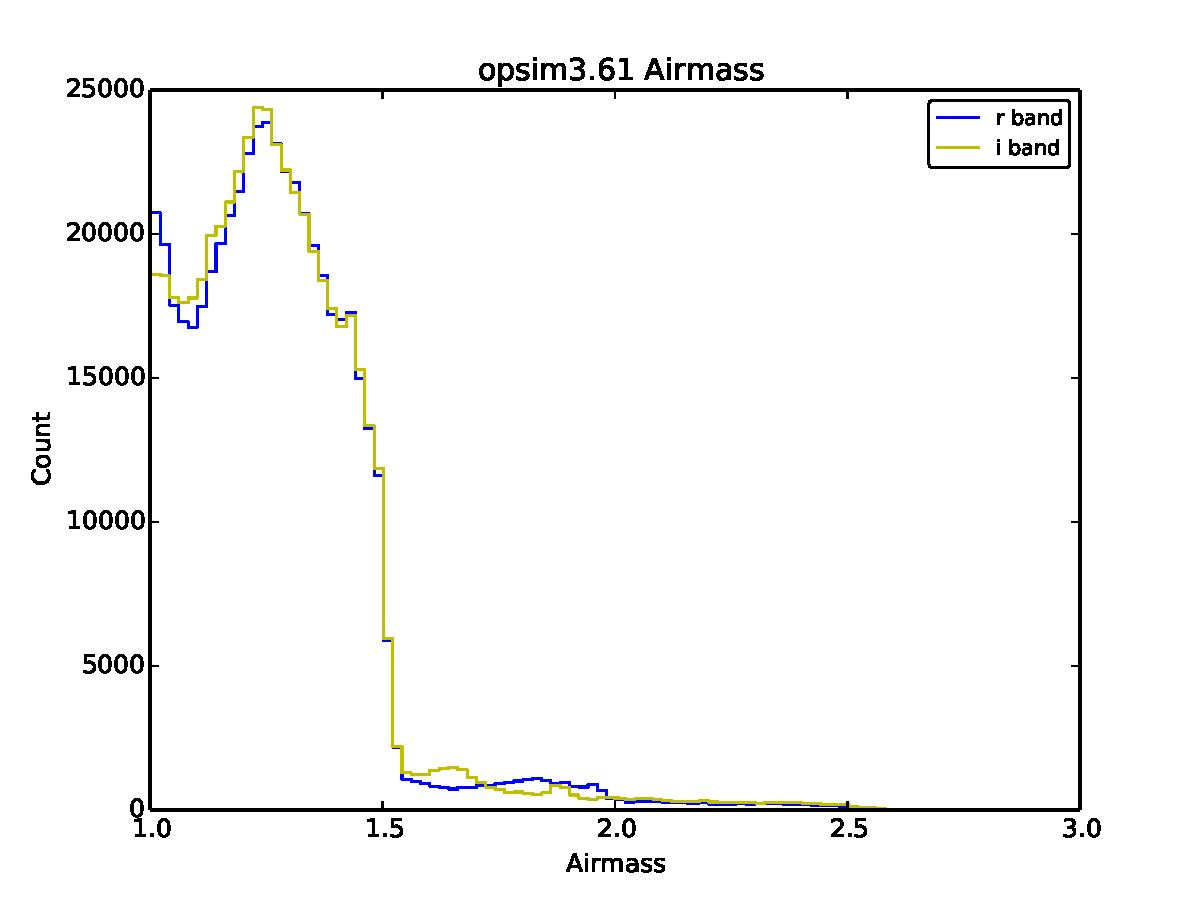
\includegraphics[height=5cm]{figures/opsim3_61__opsim3_61_Airmass_ONED_Histogram}
\caption[]
{ \label{fig:OneD}Example of using a {\tt OneDSlicer} together with a
  {\tt CountMetric} to generate a histogram of the airmass distribution in r and i
bands, and merging the result using the driver configuration file. 
}
\end{figure}

\begin{figure}
\centering
\begin{lstlisting}[frame=single]
configList = []
filters = ('g', 'r')
for f in filters:
    # Configure a metric + a OneDSlicer so that we can count how many visits 
    #  are within in each interval of the seeing value in the OneDSlicer. 
    m1 = configureMetric('CountMetric', params=['Airmass'], kwargs={'metricName':'Airmass'},
                          # Set up a additional histogram so that the outputs of these count metrics in each
                          #   filter get combined into a single plot (with both r and i band). 
                          histMerge = {'histNum':1, 'legendloc':'upper right', 'label':'%s band' %(f),
                                       'xlabel':'Airmass', 'color':colors[f]})
    # Set up the OneDSlicer, including setting the interval size for slicing.
    slicer = configureSlicer('OneDSlicer', kwargs={'sliceColName':'Airmass', 'slicesize':0.02},
                              metricDict=makeDict(m1), constraints=['filter = "%s"' %(f)])
    configList.append(slicer)
\end{lstlisting}
\caption[]
{\label{fig:oneDdriver}These configuration lines let us loop over
  several filters, and create a histogram of the airmass distribution
  in each filter. The `histMerge' line tells the driver to merge the
  histograms into a single plot, which is shown in Figure~\ref{fig:OneD}.}
\end{figure}

Next, let us evaluate the number of visits and
the coadded limiting magnitude over the sky, this time in $g$ band,
and do this at a resolution sufficient to resolve overlaps between
LSST fields of view. At the time of this publication, the LSST OpSim uses fixed field
pointings\footnote{In the future, the OpSim will likely adopt a
dithering pattern of some kind, which will be based on evaluations of
various dither patterns by the LSST community.}, returning to the
same RA and Dec for each field every time -- however, these fields do
overlap slightly, on the order of 100 arcminutes. By using the
{\tt HealpixSlicer}, with a value of NSIDE of at least 64, we can begin to
resolve the field overlaps.  Coupling this with a {\tt CountMetric}, we can evaluate
the number of visits to each RA and Dec point in the HEALpix grid. We
can also calculate the coadded depth at each point in the HEALpix grid
using the provided {\tt Coaddm5Metric}, which uses the individual visit
5-sigma limiting magnitude output by OpSim and combines them according
to
\begin{equation}
\rm{Coadd\, m5} = 1.25 \log_{10} \sum ( 10^{0.8 \,\rm{m5_i}} ).
\end{equation}
The resulting metric values will be two arrays, containing the number of visits and the
coadded m5 values evaluated at the RA/Dec point defining each
healpixel. The {\tt HealpixSlicer} then provides the following methods to
visualize these metric values: a SkyMap (see
Figures~\ref{subfig:gbanda} and \ref{subfig:gbandb} for examples), a Histogram, where the area of each healpixel
is used to convert the histogram counts into area on the sky (see
Figures~\ref{subfig:gbandc} and \ref{subfig:gbandd}), and a Power Spectrum (see
Figures~\ref{subfig:gbande} and \ref{subfig:gbandf}). The {\tt HealpixSlicer} uses
healpy's anafast function to calculate the angular power spectrum and
plots the result, optionally removing the spherical harmonic dipole. 

\begin{figure}
\begin{center}
\begin{subfigure}[b]{0.48\textwidth}
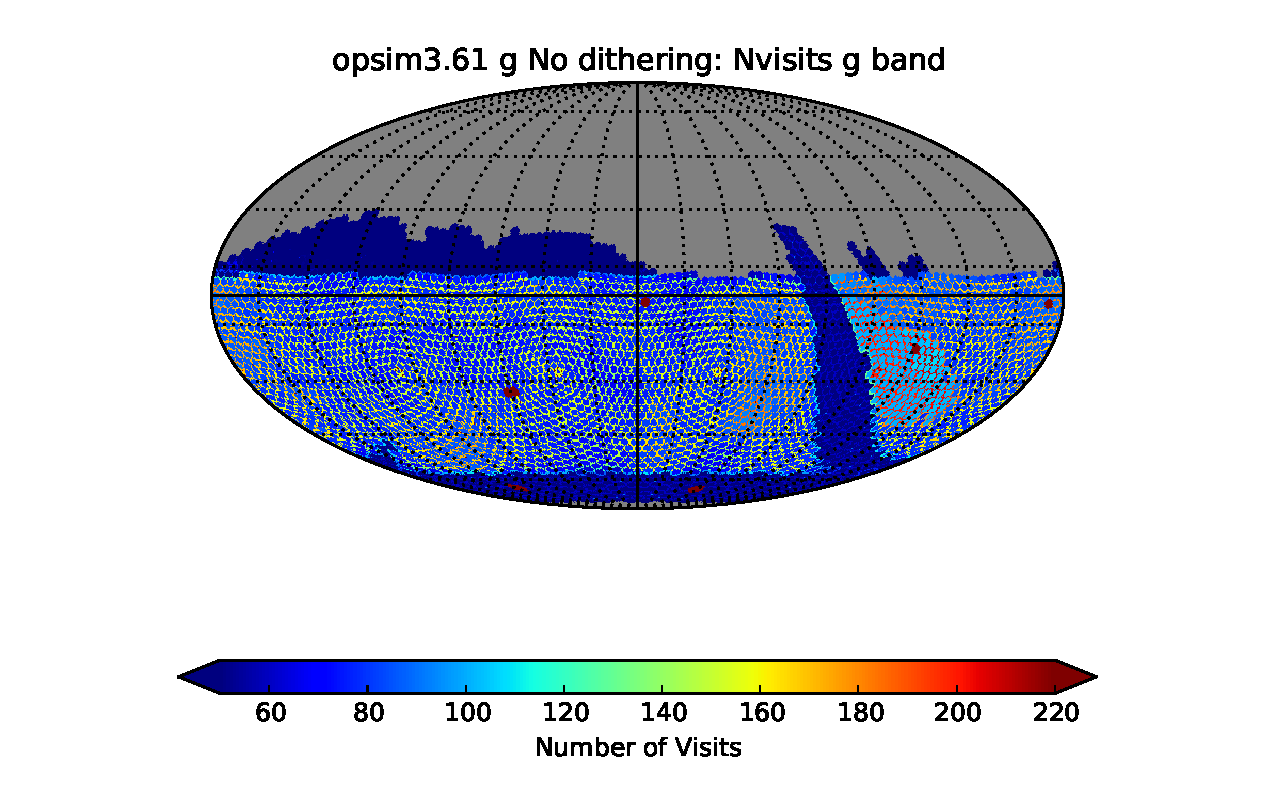
\includegraphics[width=\textwidth]{figures/opsim3_61_Nvisits_g_band_g_No_dithering_HEAL_SkyMap}
\caption{}
\label{subfig:gbanda}
\end{subfigure}
\begin{subfigure}[b]{0.48\textwidth}
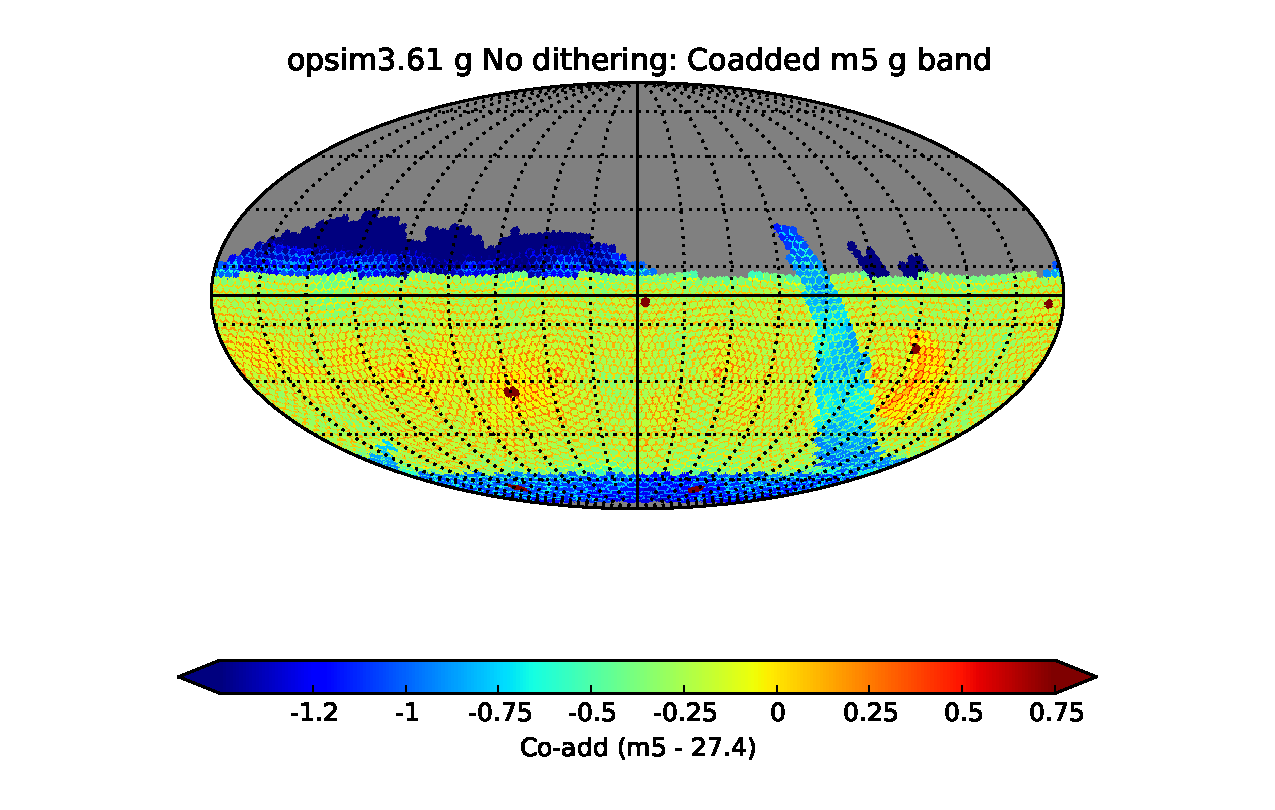
\includegraphics[width=\textwidth]{figures/opsim3_61_Coadded_m5_g_band_g_No_dithering_HEAL_SkyMap}
\caption{}
\label{subfig:gbandb}
\end{subfigure}

\begin{subfigure}[]{0.2\textwidth}
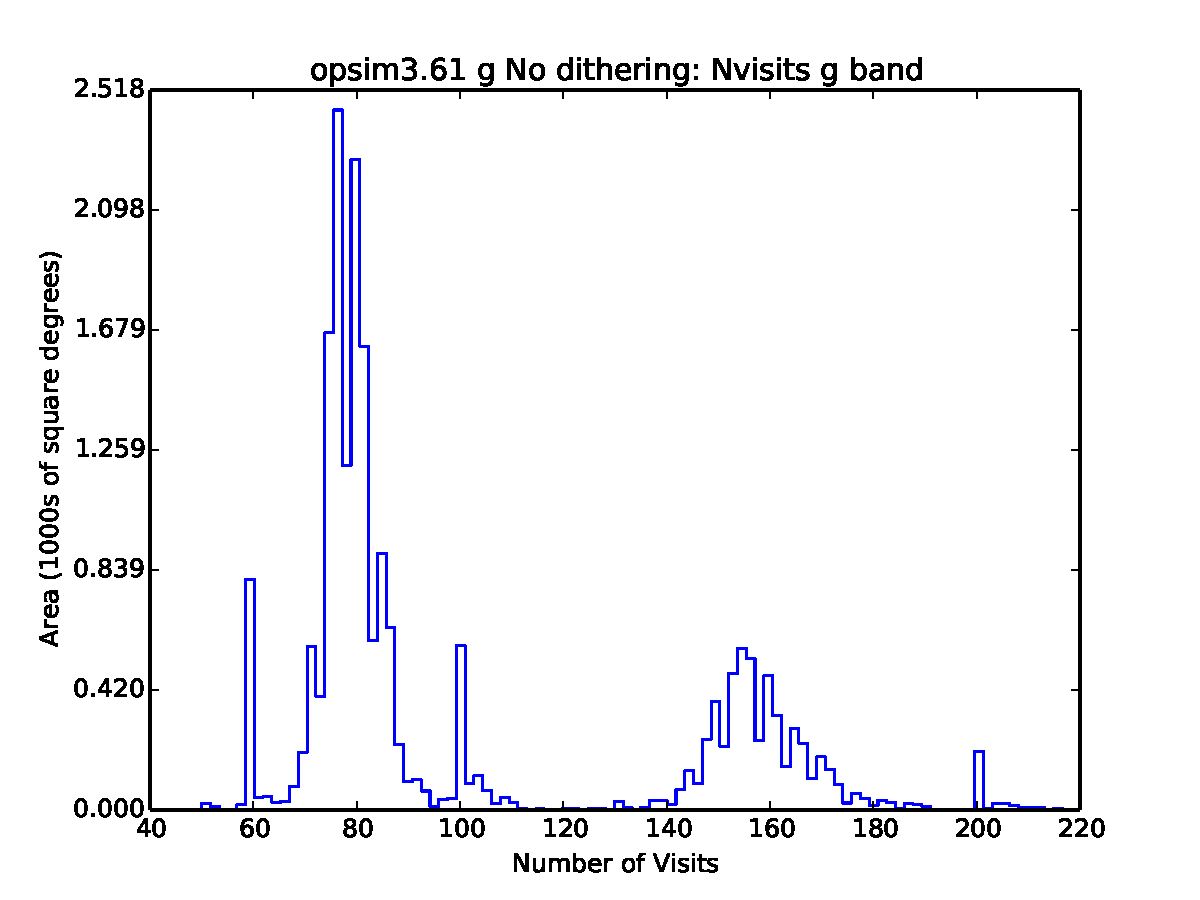
\includegraphics[width=\textwidth]{figures/opsim3_61_Nvisits_g_band_g_No_dithering_HEAL_Histogram}
\caption{}
\label{subfig:gbandc}
\end{subfigure}
\begin{subfigure}[]{0.2\textwidth}
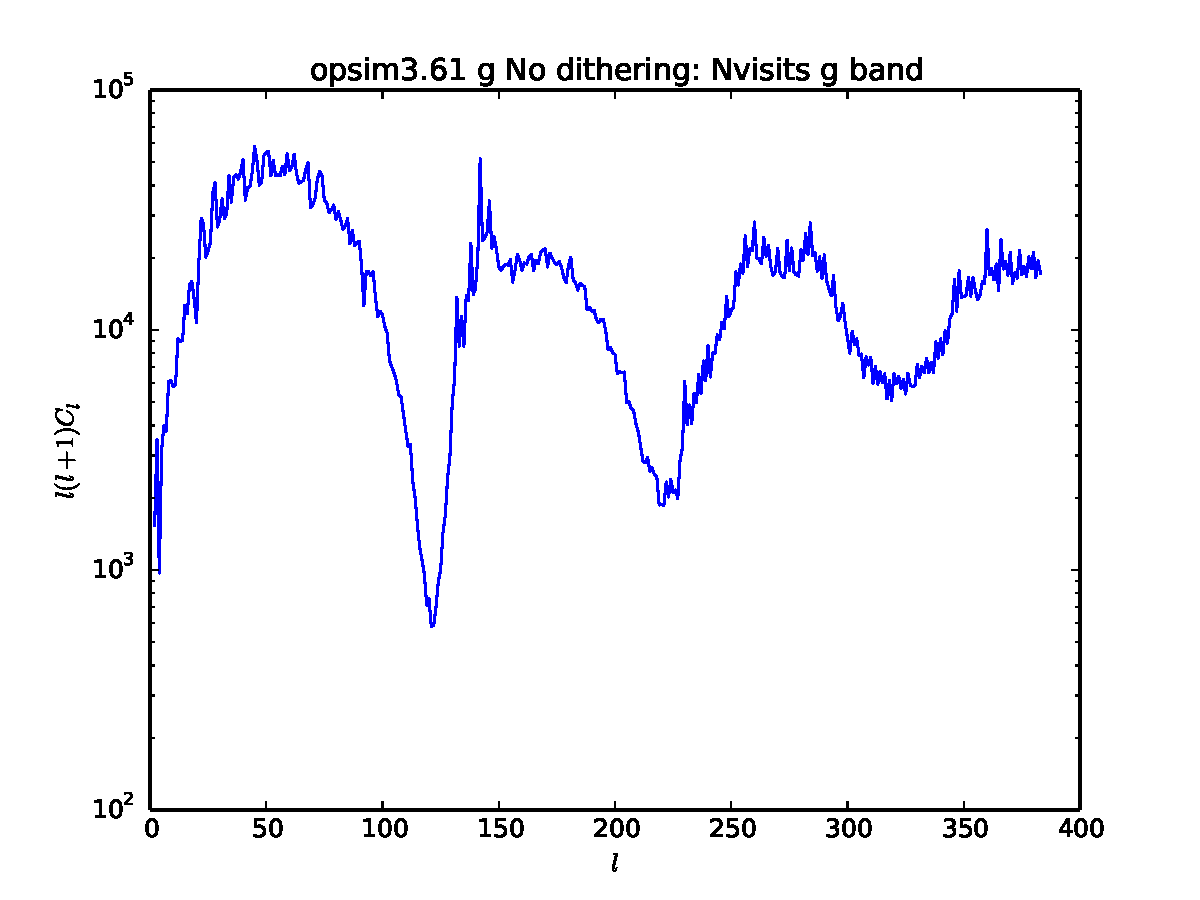
\includegraphics[width=\textwidth]{figures/opsim3_61_Nvisits_g_band_g_No_dithering_HEAL_PowerSpectrum}
\caption{}
\label{subfig:gbandd}
\end{subfigure}
~~
\begin{subfigure}[]{0.2\textwidth}
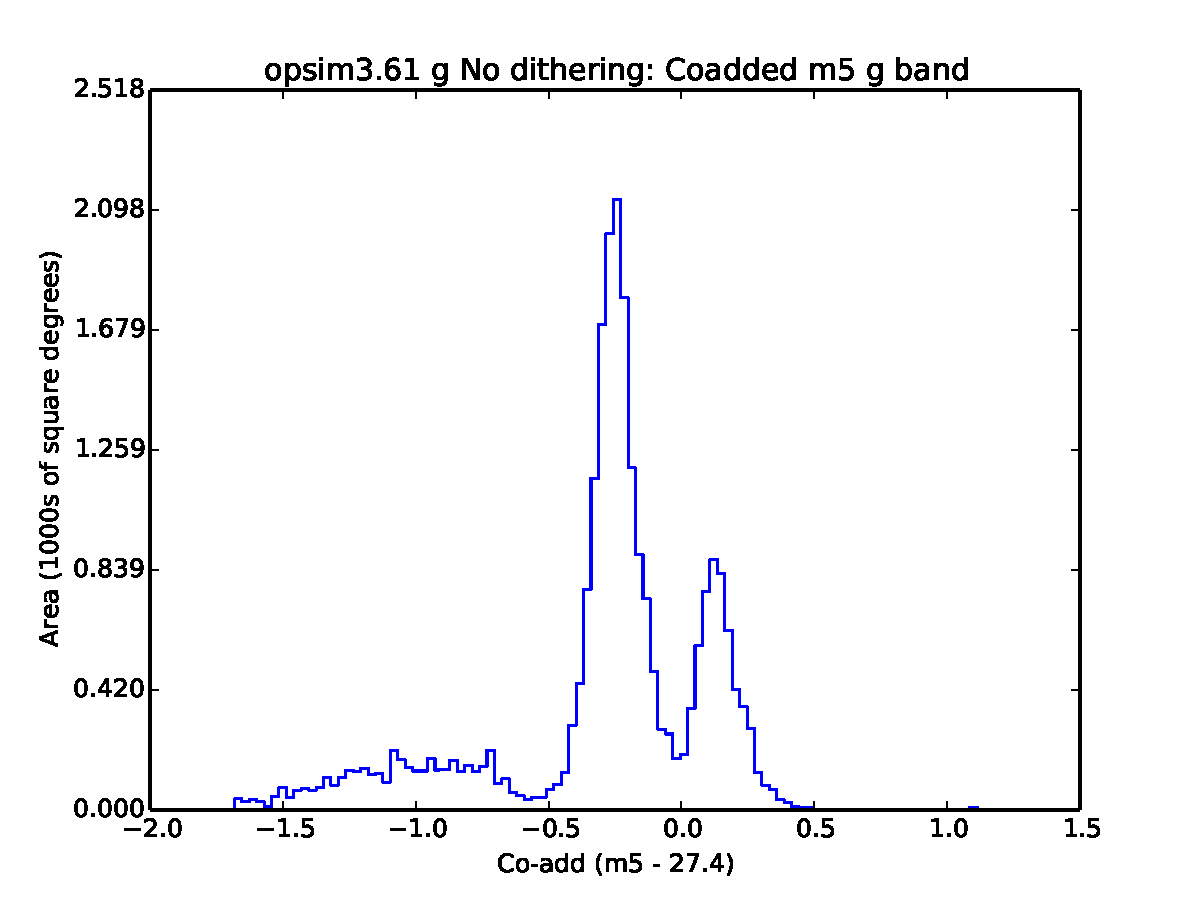
\includegraphics[width=\textwidth]{figures/opsim3_61_Coadded_m5_g_band_g_No_dithering_HEAL_Histogram}
\caption{}
\label{subfig:gbande}
\end{subfigure}
\begin{subfigure}[]{0.2\textwidth}
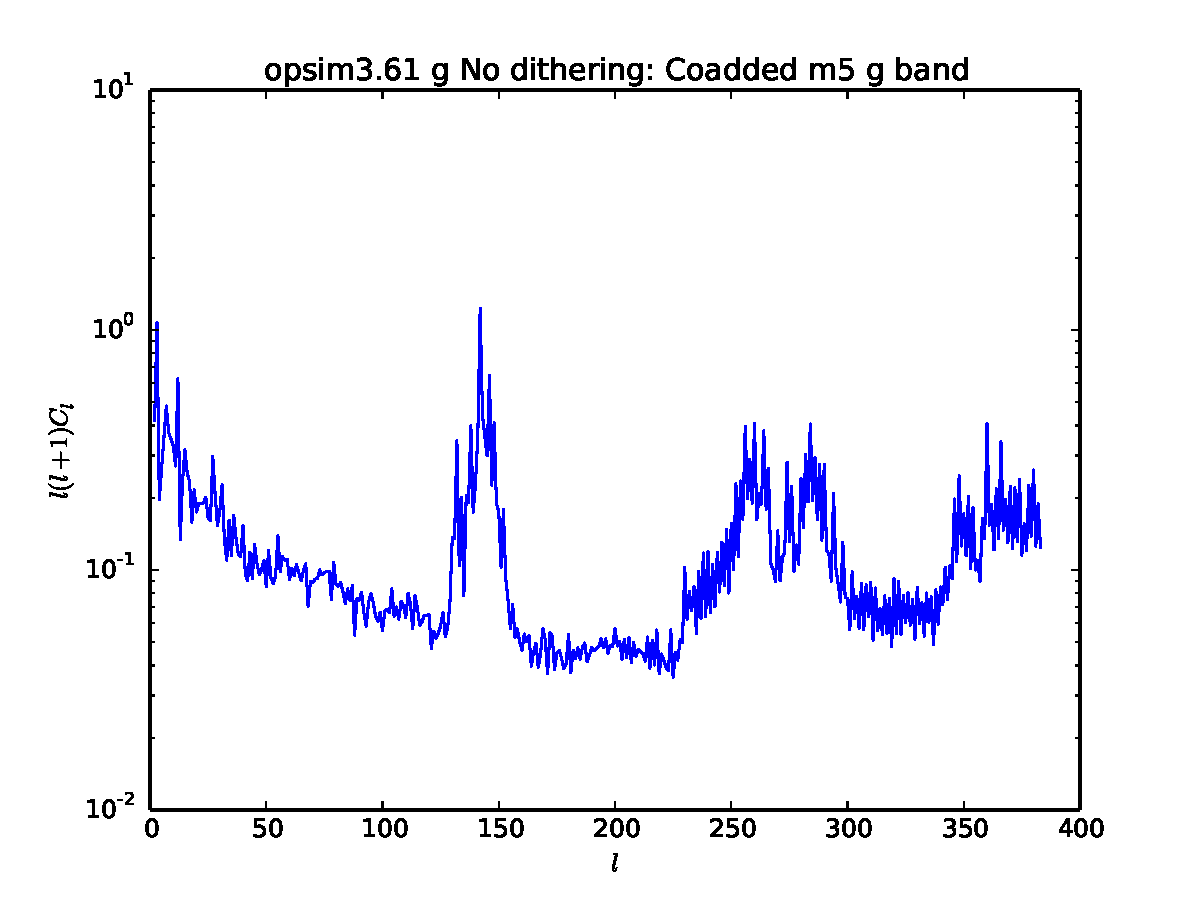
\includegraphics[width=\textwidth]{figures/opsim3_61_Coadded_m5_g_band_g_No_dithering_HEAL_PowerSpectrum}
\caption{}
\label{subfig:gbandf}
\end{subfigure}
\end{center}
\caption[]
{ \label{fig:gband}
Example of the plots resulting from using the {\tt HealpixSlicer} to calculate the number of visits per
healpixel and the coadded limiting magnitude per
healpixel. Panels~\ref{subfig:gbanda} and \ref{subfig:gbandb} show the
skymap of the number of visits and coadded depth (respectively) in $g$
band. Panels~\ref{subfig:gbandc} and \ref{subfig:gbandd} show the additional
visualizations available from the {\tt HealpixSlicer}: a histogram of the
area corresponding to a particular number of visits, and the angular
power spectrum of the number of visits across the
sky. Panels~\ref{subfig:gbande} and ~\ref{subfig:gbandf} show these
additional plots for the coadded limiting magnitude {\tt Metric}. 
}
\end{figure}

\subsection{Adding summary statistics}

We can also calculate `summary statistics' on any calculated metric
value. Summary statistics are intended to take metric values
calculated across the sky or over many intervals and extract a scalar
value as a `summary'. Any {\tt Metric} can be used to calculate a summary
statistic, as long as it only requires a single column of data (the
metric values).  We previously calculated the number of visits
and coadded depth at each HEALpix in $g$ band. In order to more easily compare
many different OpSim simulated surveys, we would want to know the mean and
rms of the distribution of these values across the sky. We can easily
do that via the {\tt Driver}, by simply adding these lines to the {\tt Metric}
configuration, as shown in Figure~\ref{fig:coaddm5metric}. For this
simulation, the mean of the $g$ band number of visits was 93.8 and the
mean of the coadded depth was 26.9, while the RobustRMS (RMS
approximated by interquartile range to reject outliers) was 20.8 visits and 0.21
mags, respectively.

\begin{figure}
\centering
\begin{lstlisting}[frame=single]
# Configure Coadded depth metric, specifying m5 column 
#  and 'metricName' (which is placed at top of plots)
m2 = makeMetricConfig('Coaddm5Metric', kwargs={'m5col':'5sigma_modified',
                                               'metricName':'Coadded m5 g band'},
                       # Specify some options for plotting - zp removes a zeropoint from plotted values
                       plotDict={'zp':mag_zpoint,
                                 'plotMin':-1.5, 'plotMax':0.75,
                                 'units':'Co-add (m5 - % .1f)'%mag_zpoint},
                       # Calculate summary statistics "mean" and "rms" 
                       summaryStats={'MeanMetric':{}, 'RobustRms':{}})
\end{lstlisting}
\caption[]
{\label{fig:coaddm5metric}Example of configuring a {\tt Metric} where
  specific plotting options are desired (in particular, here a
  zeropoint is subtracted from all metric values before plotting; a
  normalization value is also supported), and a mean and robust rms summary
  statistics are specified.}
\end{figure}

\subsection{Evaluating dithering strategies: Adding columns on the fly}

Thus far we have demonstrated how to evaluate properties of all visits
(or a subset selected by a SQL constraint) using the {\tt UniSlicer}, how to
evaluate properties of visits defined by a series of intervals using
the {\tt OneDSlicer}, and how to evaluate properties of visits at all points
across the sky (resolving field overlaps) using the {\tt HealpixSlicer}, as
well as how to summarize the results of these evaluations into a
single scalar number using summary statistics. We showed how this can
be done simply using the MAF {\tt Driver}. Next, let's consider a more
complicated analysis that includes the MAF utility to generate data
columns `on the fly' in order to evaluate some dithering strategies.

As mentioned above, the existing OpSim simulated surveys use a fixed
tesselation of the sky when scheduling visits. In the current OpSim
simulated survey outputs, the `fieldRA' and `fieldDec' columns refer
to these fixed field centers. The OpSim database outputs also provide
an example of a dithering strategy, referred to as `hexdither'. The
hexdither strategy offsets all the original fieldRA and fieldDec
values in a night by a consistent amount in RA and Dec; the size of
the offset is defined by a series of vertices, packed in a triangular
pattern into a hexagon inscribed in LSST field of view.  The resulting
RA and Dec values are recorded in the `hexdithra' and `hexdithdec'
columns in the OpSim outputs.  Figure~\ref{fig:vertices} illustrates
the pattern of the hexdither vertices within the LSST field of view;
when all 217 vertices have been visited, the pattern repeats again
from the beginning.  Evaluating other potential dithering strategies is
straightforward with MAF.

When using the {\tt HealpixSlicer}, each data slice consists of visits
overlapping the HEALpix RA/Dec point. Determining the relevant visits
is based on the visit `fieldRA' and `fieldDec' by default; however,
the {\tt HealpixSlicer} can also be configured to use other columns -- such
as the `hexdithra' and `hexdithdec' columns. Thus, it is extremely
easy to run a set of {\tt Metrics} on the original, non-dithered field
pointings and then run the same set of {\tt Metrics} using a {\tt HealpixSlicer}
configured to use the hexdithered pointings. The same is true of any
RA/Dec-like columns which are added straight into the OpSim database
file. However, MAF also provides users the capability of adding new
columns to the OpSim visit data after the data has been queried from the database. We can use this to
evaluate dithering strategies without altering the OpSim database,
instead simply writing a small amount of additional python code -- a new
MAF {\tt Stacker} class.  An example {\tt Stacker} written to
add a random RA and Dec dither to each pointing is shown in
Figure~\ref{fig:randomRADECcode}.  The framework then handles
identifying which data columns come from {\tt Stackers} and generating
the required data at runtime. Using these new
columns is simple and in the driver configuration file there is no
differentiation between columns retrieved directly from the database
or columns generated by {\tt Stackers} -- the name of the column
desired for `spatialkey1' and `spatialkey2' is simply entered into the
configureSlicer kwargs in the driver config. This can be seen in the full
driver configuration file at {\url {http://ls.st/mxl}}.

Previously we evaluated the number of visits and coadded depth in $g$
band, using a {\tt HealpixSlicer}. We can now repeat this evaluation, but
apply each of these different dithering strategies as well. The
results are shown in Figure~\ref{fig:dither_nvis_coadd}. As can be
seen, the peaks in the number of visits and coadded depth due to field
overlaps are dramatically smoothed by both the hexdither and random dither
strategies. We can also generate histograms showing the area achieving a
given number of visits and the area achieving a given coadded depth
(see Panels~\ref{subfig:nvis_hist} and \ref{subfig:coadd_hist}), which
show that the double peaks in coadded depth corresponding to field
centers vs. field overlaps are smoothed into a single peak. Similarly, we can
create plots to compare the power spectra; Panel~\ref{subfig:coadd_ps}
shows the dramatic difference that dithering makes. In the
non-dithered case, the peaks in the power spectra of the coadded depth
can print through to galaxy number counts, causing problems for large
scale structure cosmological analysis\cite{Carroll}.

\begin{figure}
\centering
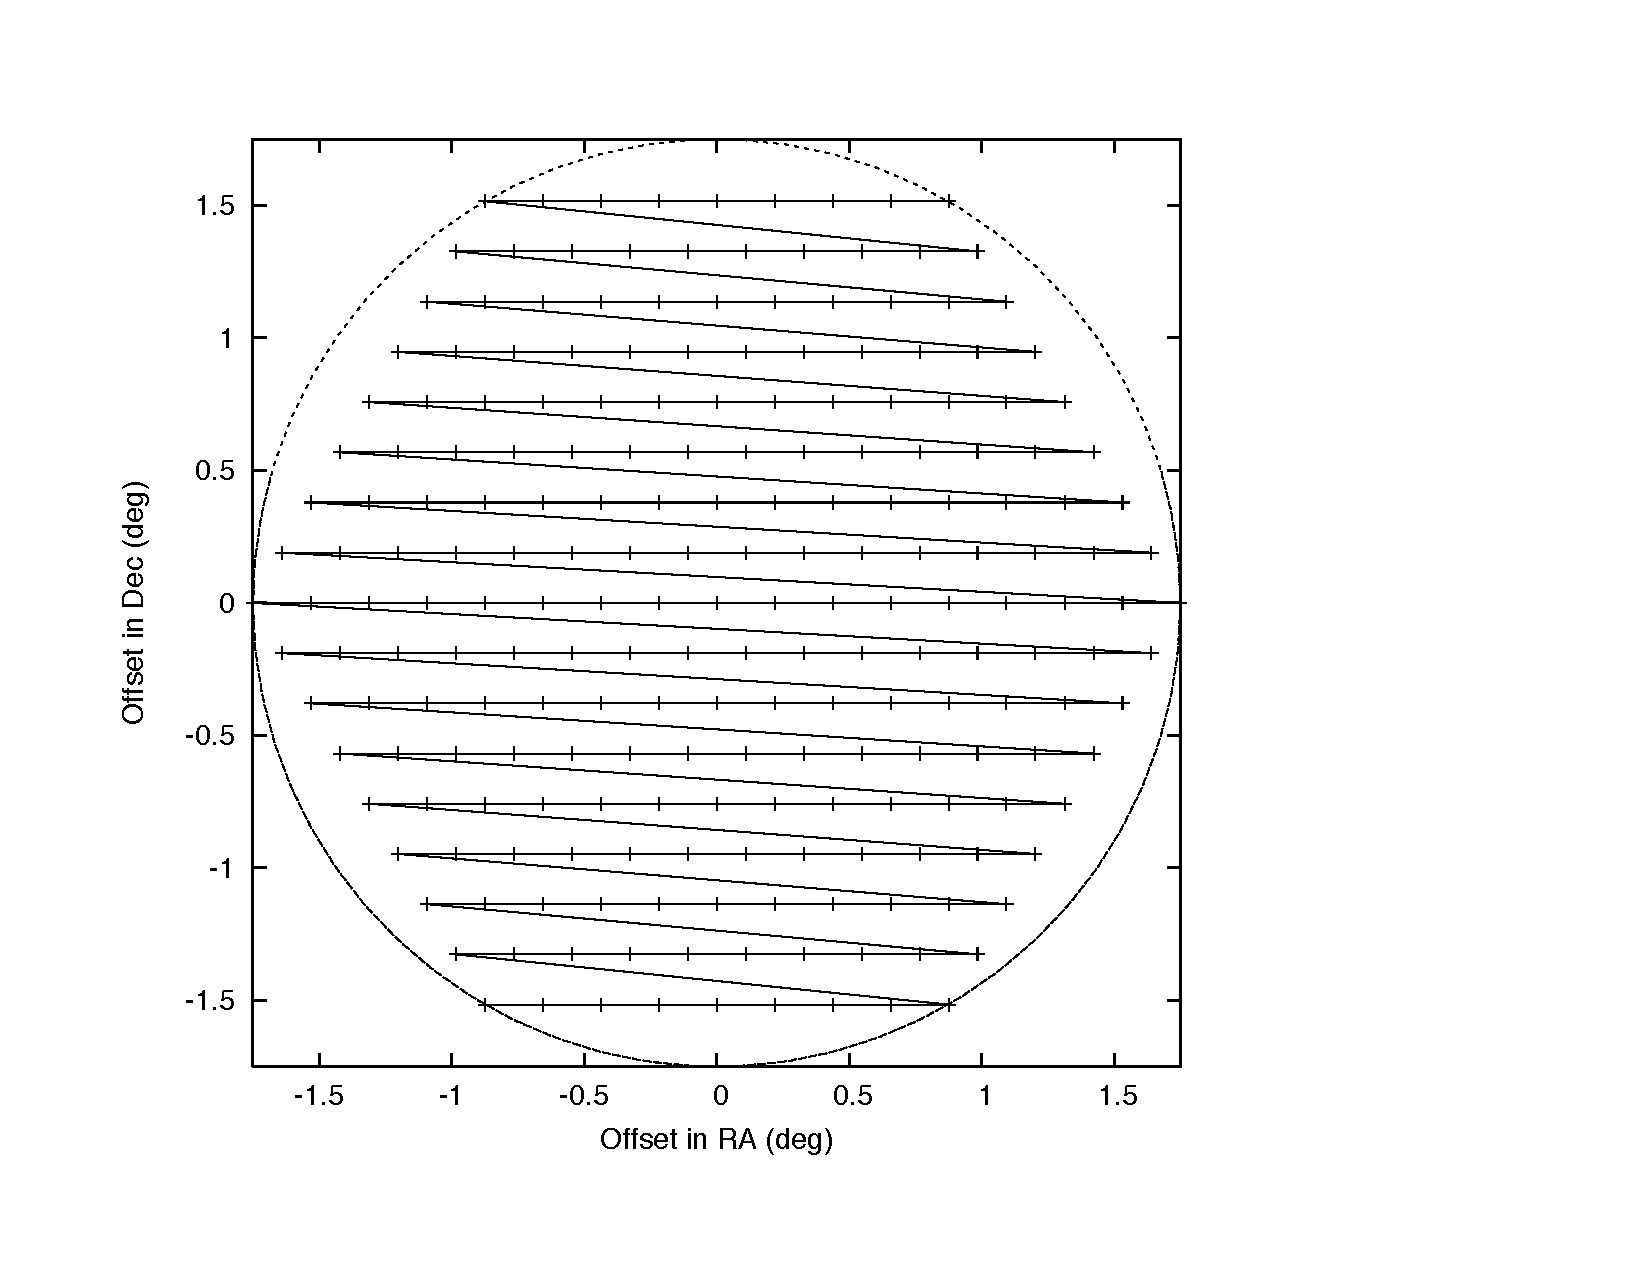
\includegraphics[width=0.4\textwidth]{figures/dither_vert}
\caption[]
{\label{fig:vertices}
The hexdither dithering strategy offsets the fixed OpSim field centers
by a given amount each night. The offset corresponds to the vertexes
of a triangular tesselation of the hexagon inscribed in the LSST field
of view. The solid line shows the progression through the vertices by
night, from the lower left to the upper right. The offsets repeat
after the entire pattern is completed. }
\end{figure}

\begin{figure}
\centering
\begin{lstlisting}[frame=single]
class RandomDitherStacker(BaseStacker):
    """Randomly dither the RA and Dec pointings up to maxDither degrees from center."""
    def __init__(self, raCol='fieldRA', decCol='fieldDec', maxDither=1.8, randomSeed=None):
        # Instantiate the RandomDither object and set internal
variables.  
        self.raCol = raCol
        self.decCol = decCol
        self.maxDither = maxDither * np.pi / 180.0
        self.randomSeed = randomSeed
        # self.units used for plot labels. 
        self.units = 'rad'
        # Values required for framework operation: this specifies the
names of the new columns. 
        self.colsAdded = ['randomRADither', 'randomDecDither']
        # Values required for framework operation: this specifies the
data columns required from the database. 
	self.colsReq = [self.raCol, self.decCol]

    def run(self, simData):
        # Generate random numbers for dither, using defined seed value
if desired. 
        if self.randomSeed is not None:
            np.random.seed(self.randomSeed)
        dithersRA = np.random.rand(len(simData[self.raCol]))
        dithersDec = np.random.rand(len(simData[self.decCol]))
        # np.random.rand returns numbers in [0, 1) interval.                                                                                                                    
        # Scale to desired +/- maxDither range. 
        dithersRA = dithersRA*np.cos(simData[self.decCol])*2.0*self.maxDither - self.maxDither
        dithersDec = dithersDec*2.0*self.maxDither - self.maxDither
        # Add to RA and wrap back into expected range.  
        randomRADither = simData[self.raCol] + dithersRA
        randomRADither = randomRADither % (2.0*np.pi)
        # Add to Dec and wrap back into expected range.  
        randomDecDither = simData[self.decCol] + dithersDec
        randomDecDither = np.where(randomDecDither < -np.pi/2.0, -1.*(np.pi+randomDecDither), randomDecDither)
        randomDecDither = np.where(randomDecDither > np.pi/2.0, (np.pi-randomDecDither), randomDecDither)
        self.stackerCols = np.core.records.fromarrays([randomRADither, randomDecDither],
                                                      names=['randomRADither', 'randomDecDither'])
        # Add the new columns into the opsim simulated survey data.
        simData = self._opsimStack(simData)
	return simData

\end{lstlisting}
\caption[]
{\label{fig:randomRADECcode} Example {\tt Stacker} written to add a random RA
  and Dec dither to each visit pointing. The MAF {\tt Driver} uses
  these {\tt Stacker} classes to generate the additional columns at
  runtime, if the new columns are used in the driver configuration
  script. A {\tt HealpixSlicer} can be easily configured to use
these new dithering columns generated on the fly within MAF by just referring
to their names in the driver configuration file. }
\end{figure}

\begin{figure}
\centering
\begin{subfigure}[]{0.3\textwidth}
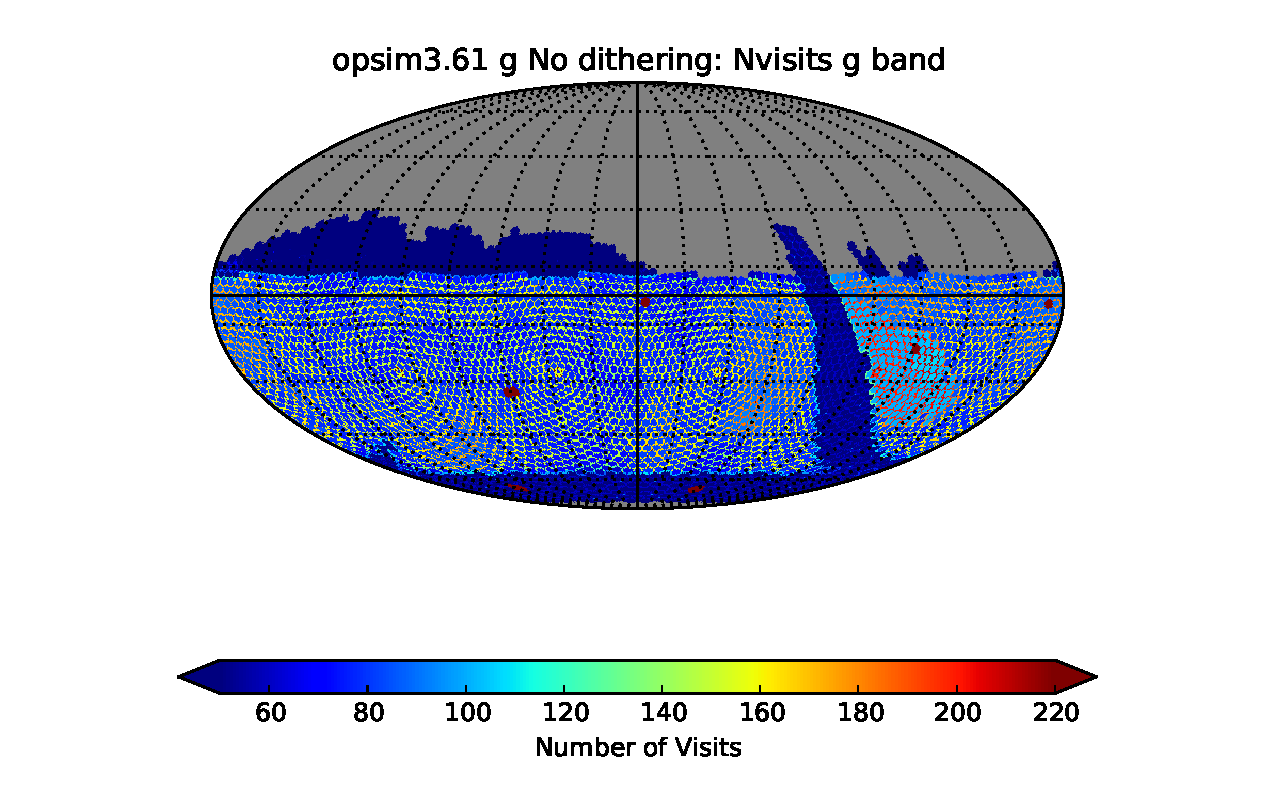
\includegraphics[width=\textwidth]{figures/opsim3_61_Nvisits_g_band_g_No_dithering_HEAL_SkyMap}
\caption[]{}
\label{subfig:nvisgno}
\end{subfigure}
\begin{subfigure}[]{0.3\textwidth}
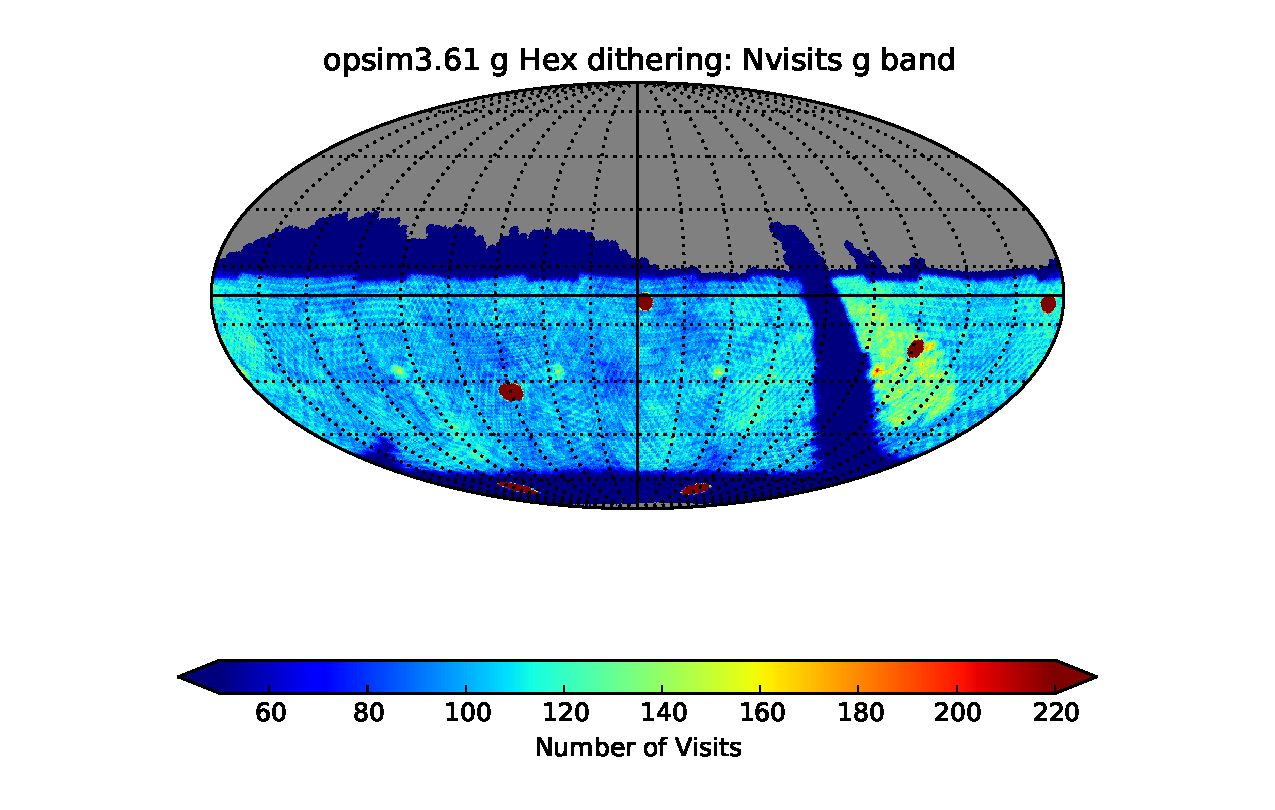
\includegraphics[width=\textwidth]{figures/opsim3_61_Nvisits_g_band_g_Hex_dithering_HEAL_SkyMap}
\caption[]{}
\label{subfig:nvisghex}
\end{subfigure}
\begin{subfigure}[]{0.3\textwidth}
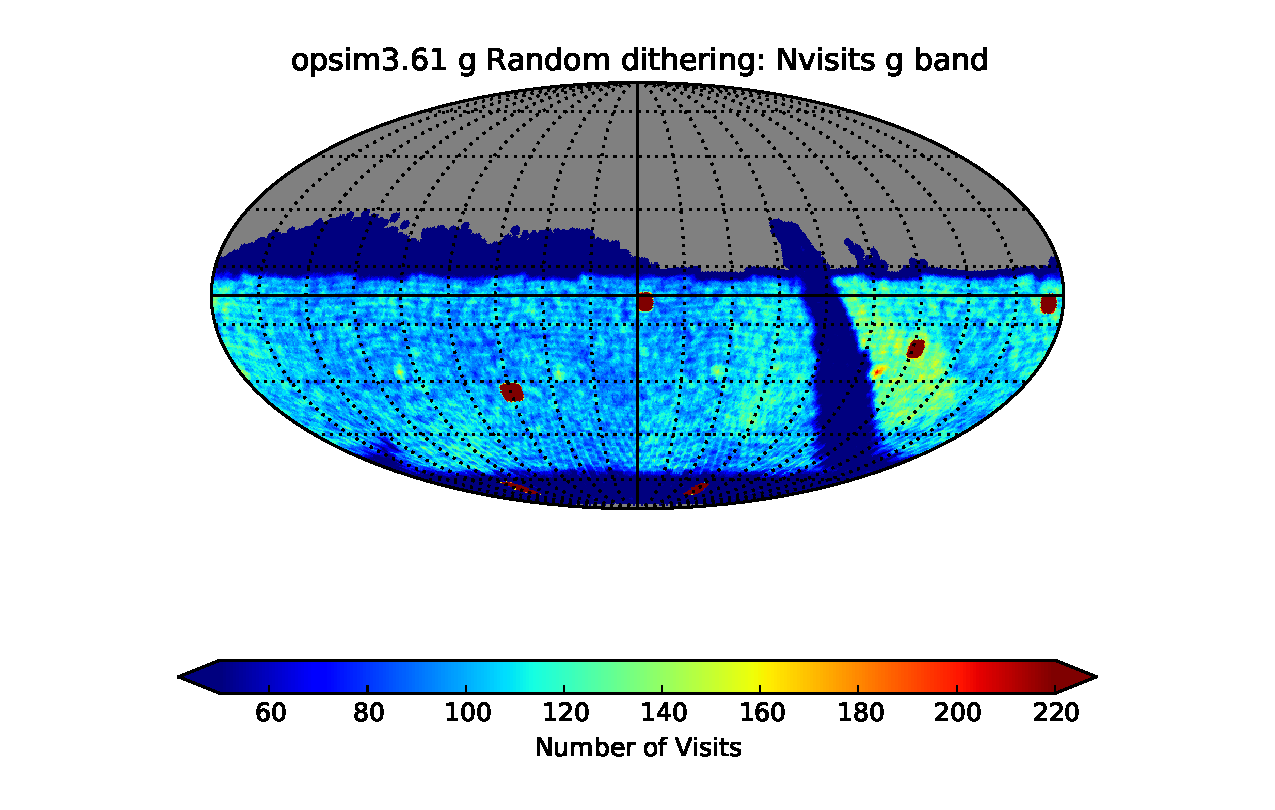
\includegraphics[width=\textwidth]{figures/opsim3_61_Nvisits_g_band_g_Random_dithering_HEAL_SkyMap}
\caption[]{}
\label{subfig:nvisgrandom}
\end{subfigure}

\begin{subfigure}[]{0.3\textwidth}
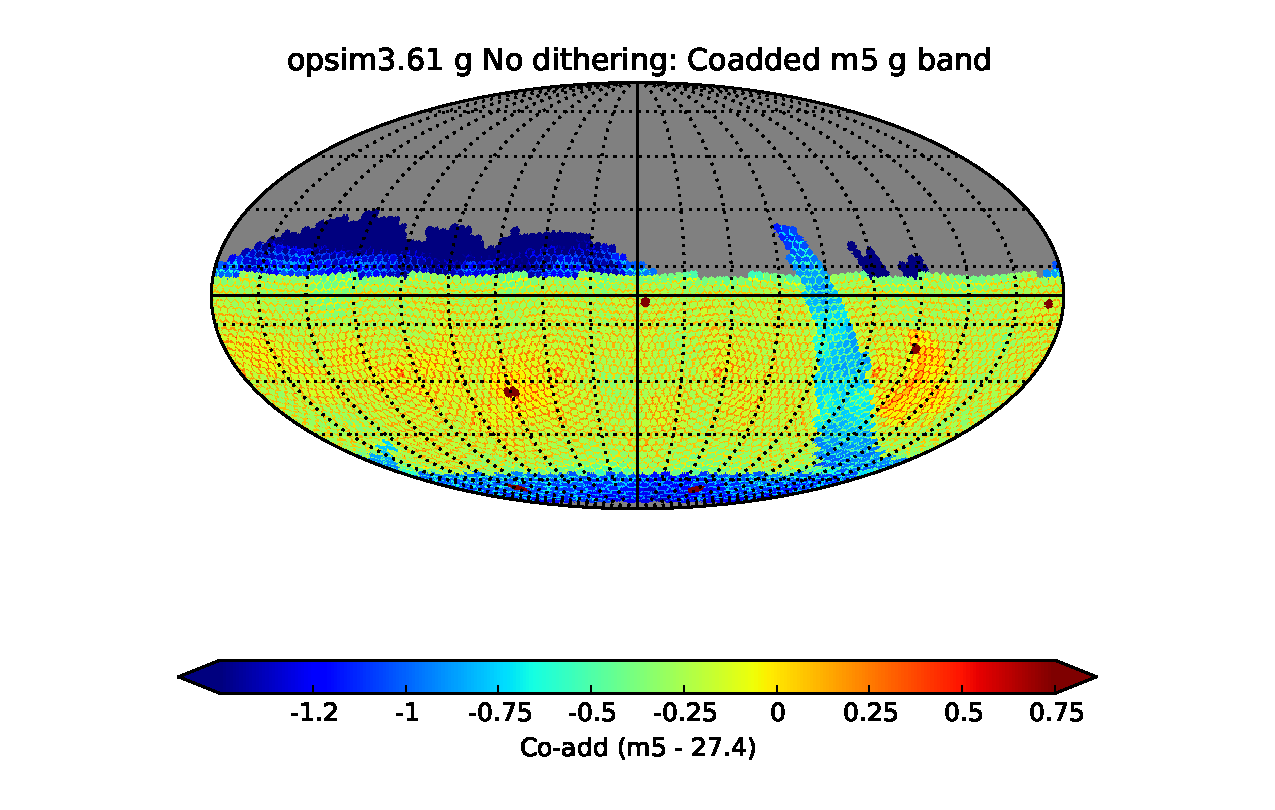
\includegraphics[width=\textwidth]{figures/opsim3_61_Coadded_m5_g_band_g_No_dithering_HEAL_SkyMap}
\caption[]{}
\label{subfig:coaddgno}
\end{subfigure}
\begin{subfigure}[]{0.3\textwidth}
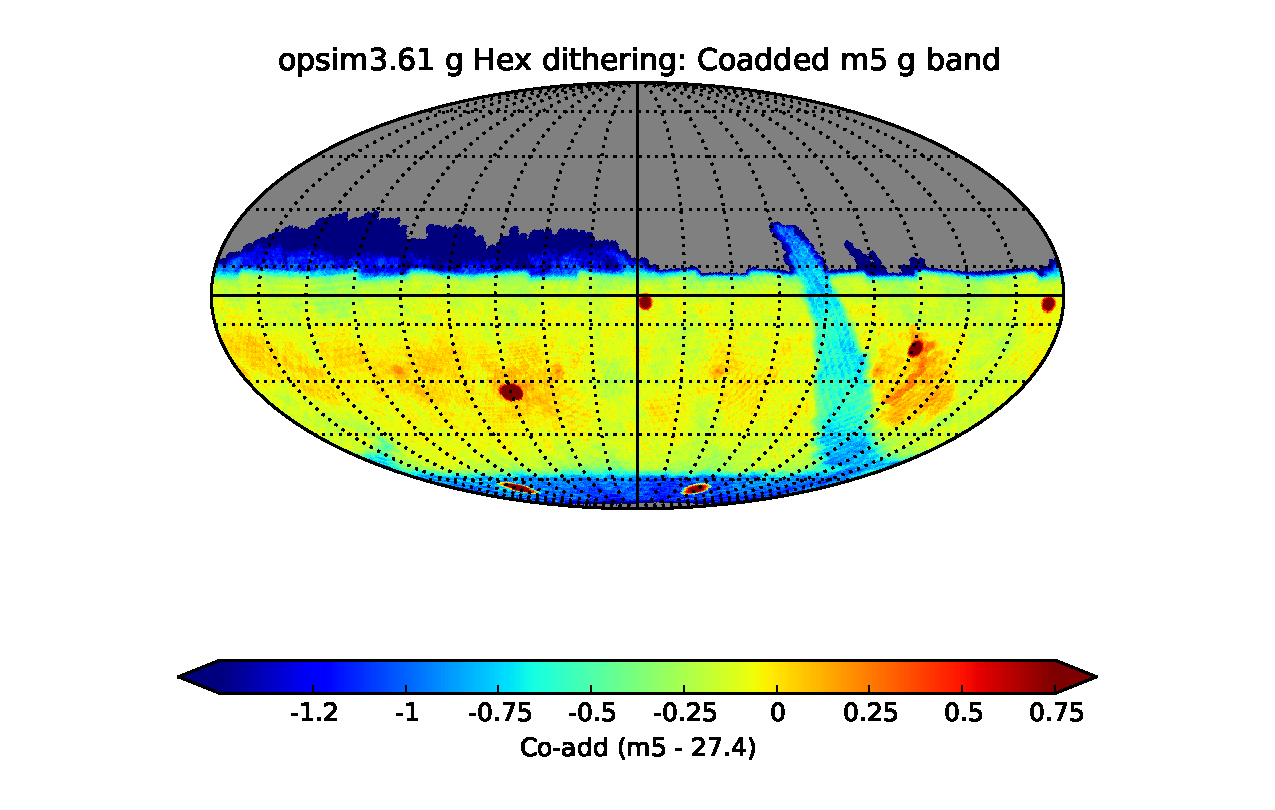
\includegraphics[width=\textwidth]{figures/opsim3_61_Coadded_m5_g_band_g_Hex_dithering_HEAL_SkyMap}
\caption[]{}
\label{subfig:coaddghex}
\end{subfigure}
\begin{subfigure}[]{0.3\textwidth}
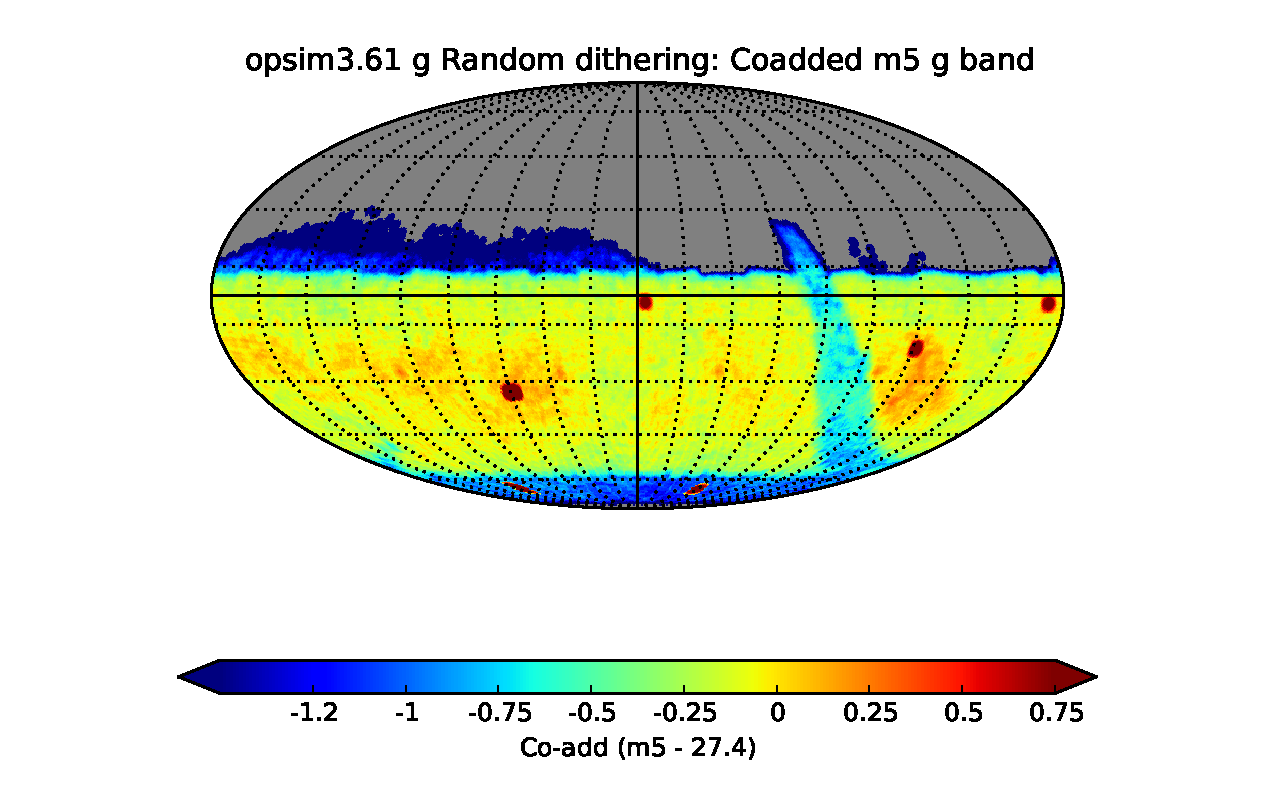
\includegraphics[width=\textwidth]{figures/opsim3_61_Coadded_m5_g_band_g_Random_dithering_HEAL_SkyMap}
\caption[]{}
\label{subfig:coaddgrandom}
\end{subfigure}

\begin{subfigure}[]{0.3\textwidth}
\centering
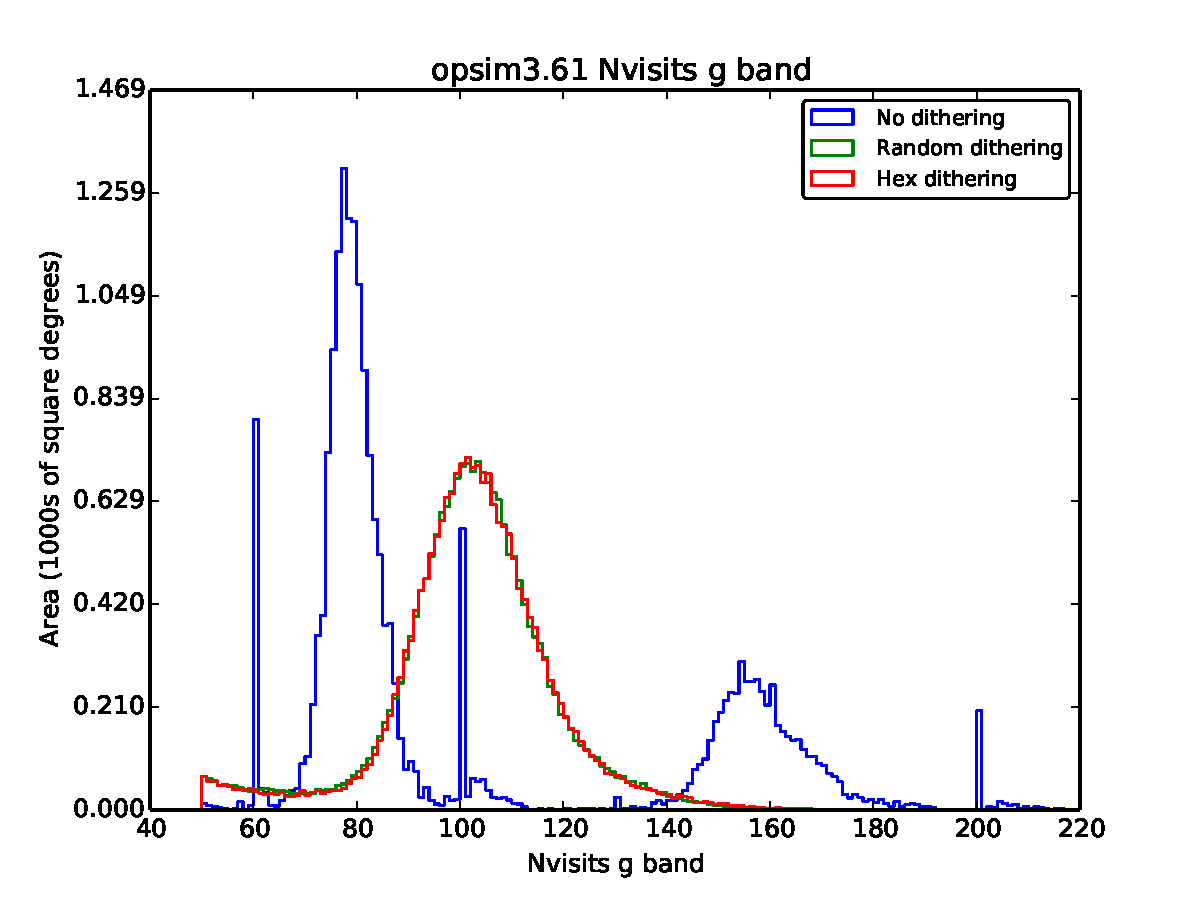
\includegraphics[width=.8\textwidth]{figures/opsim3_61__opsim3_61_Nvisits_g_band_HEAL_Histogram}
\caption[]{}
\label{subfig:nvis_hist}
\end{subfigure}
\begin{subfigure}[]{0.3\textwidth}
\centering
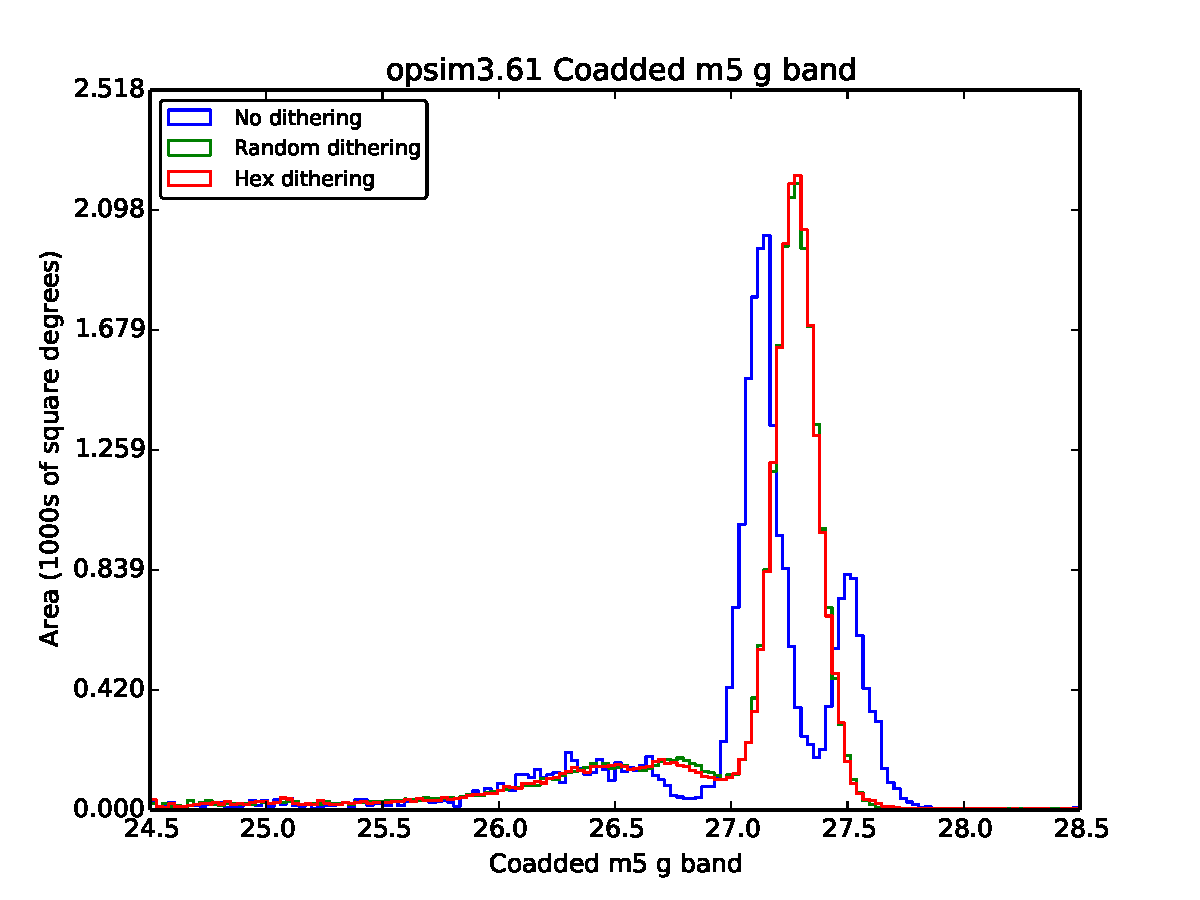
\includegraphics[width=.8\textwidth]{figures/opsim3_61__opsim3_61_Coadded_m5_g_band_HEAL_Histogram}
\caption[]{}
\label{subfig:coadd_hist}
\end{subfigure}
\begin{subfigure}[]{0.3\textwidth}
\centering
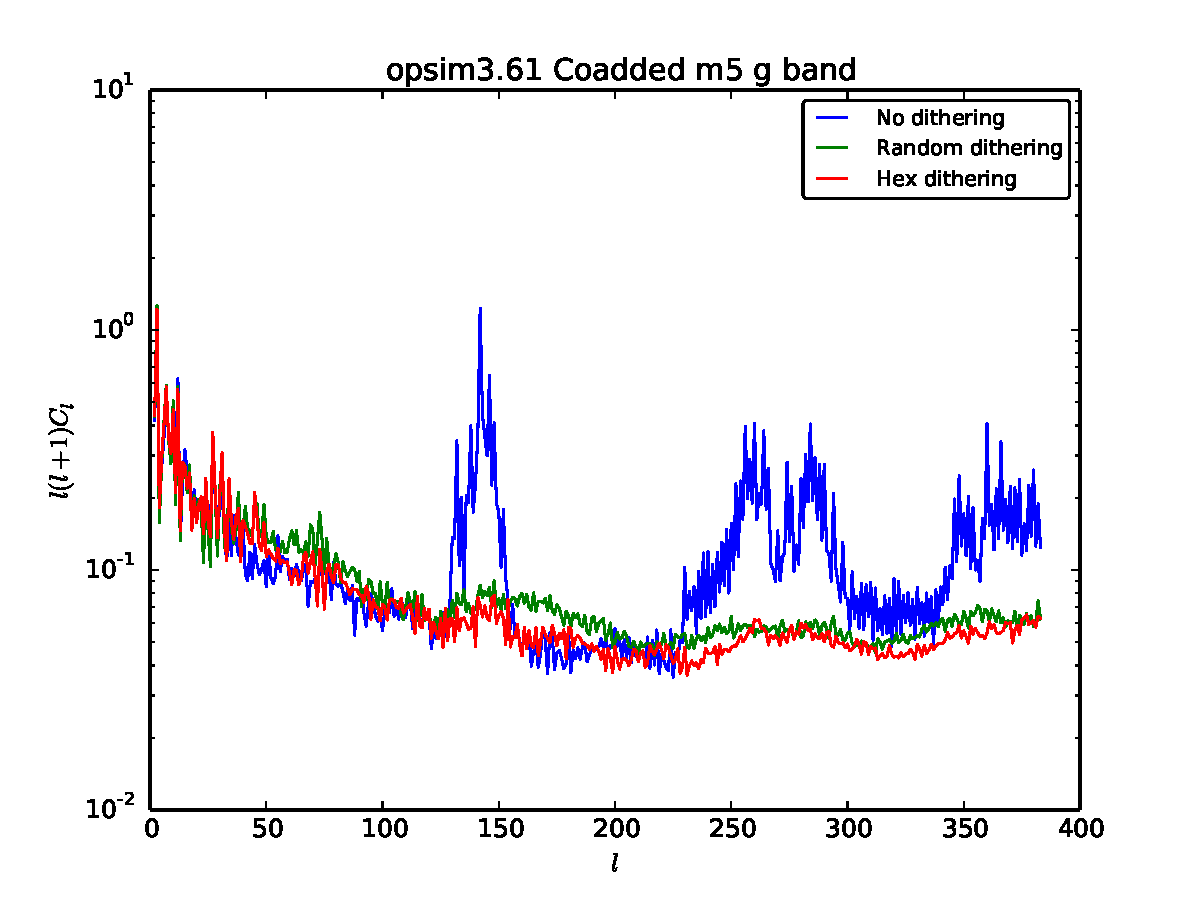
\includegraphics[width=.8\textwidth]{figures/opsim3_61__opsim3_61_Coadded_m5_g_band_HEAL_PowerSpectrum}
\caption[]{}
\label{subfig:coadd_ps}
\end{subfigure}
\caption[]
{\label{fig:dither_nvis_coadd}
Evaluating the number of visits and coadded limiting magnitude in $g$
band, in the case of no dithering (Panels~\ref{subfig:nvisgno} and
\ref{subfig:coaddgno}), hex dithering (Panels~\ref{subfig:nvisghex}
and \ref{subfig:coaddghex}) and random dithering
(Panels~\ref{subfig:nvisgrandom} and \ref{subfig:coaddgrandom})
applied to the OpSim FieldRA and FieldDec values. In the no dither and
hex dither case, the relevant RA/Dec columns are provided by the OpSim
database; the random dither RA/Dec columns were generated on the fly
using a {\tt Stacker}. Panels~\ref{subfig:nvis_hist},
\ref{subfig:coadd_hist} and \ref{subfig:coadd_ps} show the histogram
and power spectrum plots created from these metric values. The areas
with fewer visits (in the plane of the Milky Way, near the south
celestial pole, and north of
$\approx 10^{\circ}$) are areas
outside the main footprint of LSST and are observed with a different
set of requirements, including fewer visits. The six dark red circular
areas visible in the number of visits and coadded depth plots
represent the deep drilling fields, and are again observed with a
different set of requirements than the main survey. Examining
panels~\ref{subfig:coadd_ps}, we see that dithering
is extremely important for smoothing the peaks in the power spectrum
of the coadded depth, which can print through to cosmological analysis
such as galaxy clustering. It is also important for the coadded depth;
although the mean value of the coadded limiting magnitude does not
change significantly (26.98/26.99/26.98 in no dither/hex dither/random
dither, respectively) the median does increase from 27.13 without
dithering to 27.23 in both dithering options. (See Table~\ref{tab:summarystats}).}
\end{figure}

To continue this evaluation of dithering strategies a little further,
let us add a few additional {\tt Metrics}. While there are endless
possibilities, for reasons of space here we will consider only the
{\tt ProperMotion Metric} and the {\tt QuickRevisit Metric}. The {\tt ProperMotionMetric}
calculates the expected final precision in the proper motion measurement at a
given RA/Dec, based on the astrometric uncertainties in each observation
(estimated from the user-specified star's magnitude plus the 5-sigma
limiting magnitude of each visit, including an error floor) and the
times of the observations (visits spread further apart in time will
have a lower error in the proper motion), and assuming no parallax.  The
{\tt QuickRevisitMetric} simply counts the number of nights that have more
than a user-defined number of visits, a relevant statistic for
studies of variables and transients with short timescales and to solar
system object detection (although it is definitely not a comprehensive
evaluation). The {\tt QuickRevisitMetric} is just intended to be a
simple way to start looking at the effect of dithering on short
time-scale revisits (as this dithering can affect the field overlap
region, which can act as a source for significant numbers of quick
revisits). We ran the {\tt ProperMotionMetric} with stars at 20th and 24th
magnitude (to evaluate high and low SNR regimes), and looked for
nights with more than 10 visits with the
{\tt QuickRevisitMetric}. Figure~\ref{fig:dither_pm_revis} shows the results
with each of the different dithering strategies -- no dithering, hex
dithering, and random dithering. At 20th magnitude, the
{\tt ProperMotionMetric} shows very little difference between any of these
observing strategies, but once we reach 24th magnitude, it is apparent
that dithering smoothes the accuracy of the proper motion
measurements across the sky in a similar fashion to how dithering smoothed the
number of visits and coadded depth in $g$ band, above. However, it is
only when we start to consider the {\tt QuickRevisitMetric} that the
differences between the hexdither and random dither start to become
apparent. Looking at Panels~\ref{subfig:revisitno},
\ref{subfig:revisithex}, \ref{subfig:revisitrandom}, and particularly
\ref{subfig:revisithist}, we can see that in the case of no dithering,
a small area of the sky receives a large number of nights with more
than 10 visits per night. These large numbers of revisits are
due to both the Deep Drilling observations and the field
overlaps. However, with no dithering at all, most of the sky receives much fewer than 5
nights with 10 or more visits within any night. Meanwhile, random dithering (where
each visit is independently and randomly dithered) spreads visits
around the sky, so no significant portion of sky has more than 20
nights with more than 10 visits -- but the average patch of sky
receives a larger number of nights with 10 or more revisits; i.e., the median number of nights with
at least 10 revisits is higher than with no dithering. Hexdither, on the other hand, because it
keeps a constant offset from the original fixed field pointings for an
entire night (thus preserving field overlaps within a night, while
still smoothing the location of the overlaps from one night to the
next), has an even higher median number of nights with 10 or more
revisits. This is reflected in the summary statistics for this {\tt Metric},
see Table~\ref{tab:summarystats}. 

\begin{figure}
\centering
\begin{subfigure}[]{0.3\textwidth}
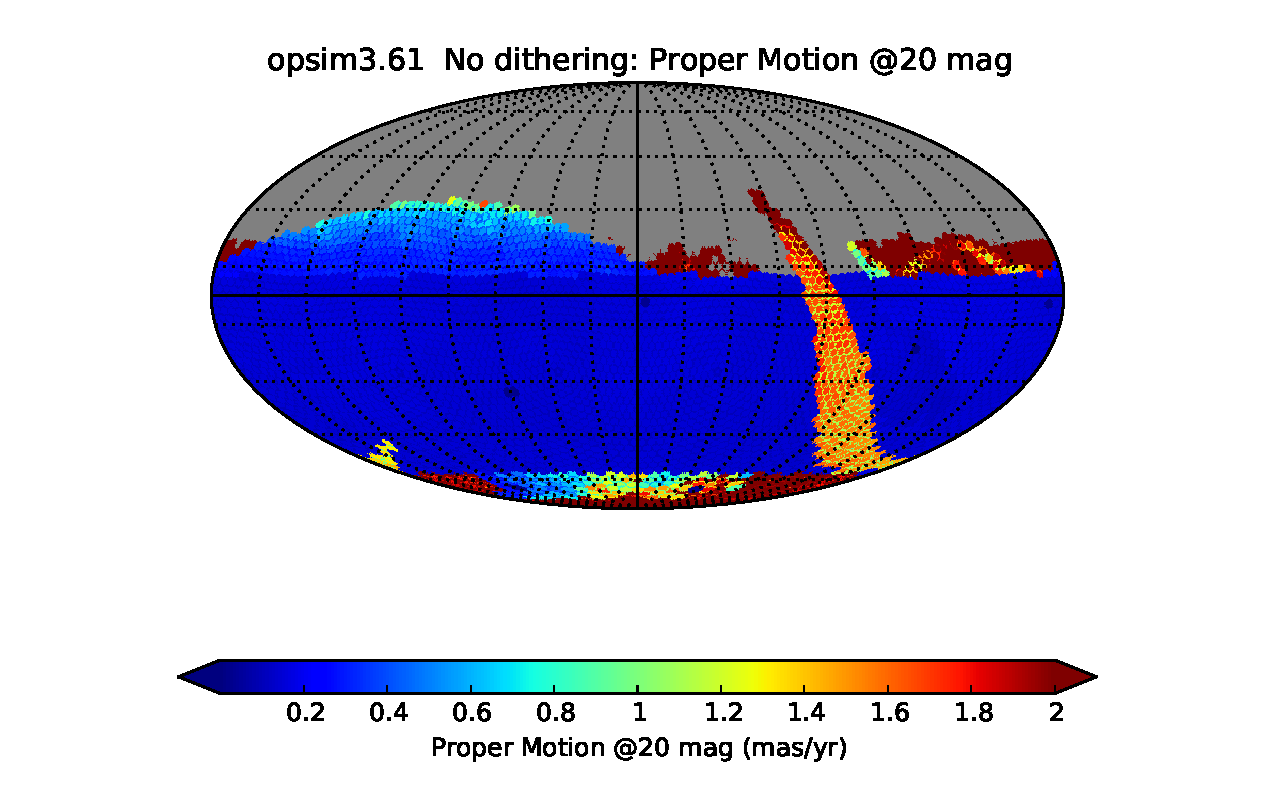
\includegraphics[width=\textwidth]{figures/opsim3_61_Proper_Motion_@20_mag__No_dithering_HEAL_SkyMap}
\caption[]{}
\label{subfig:pm20no}
\end{subfigure}
\begin{subfigure}[]{0.3\textwidth}
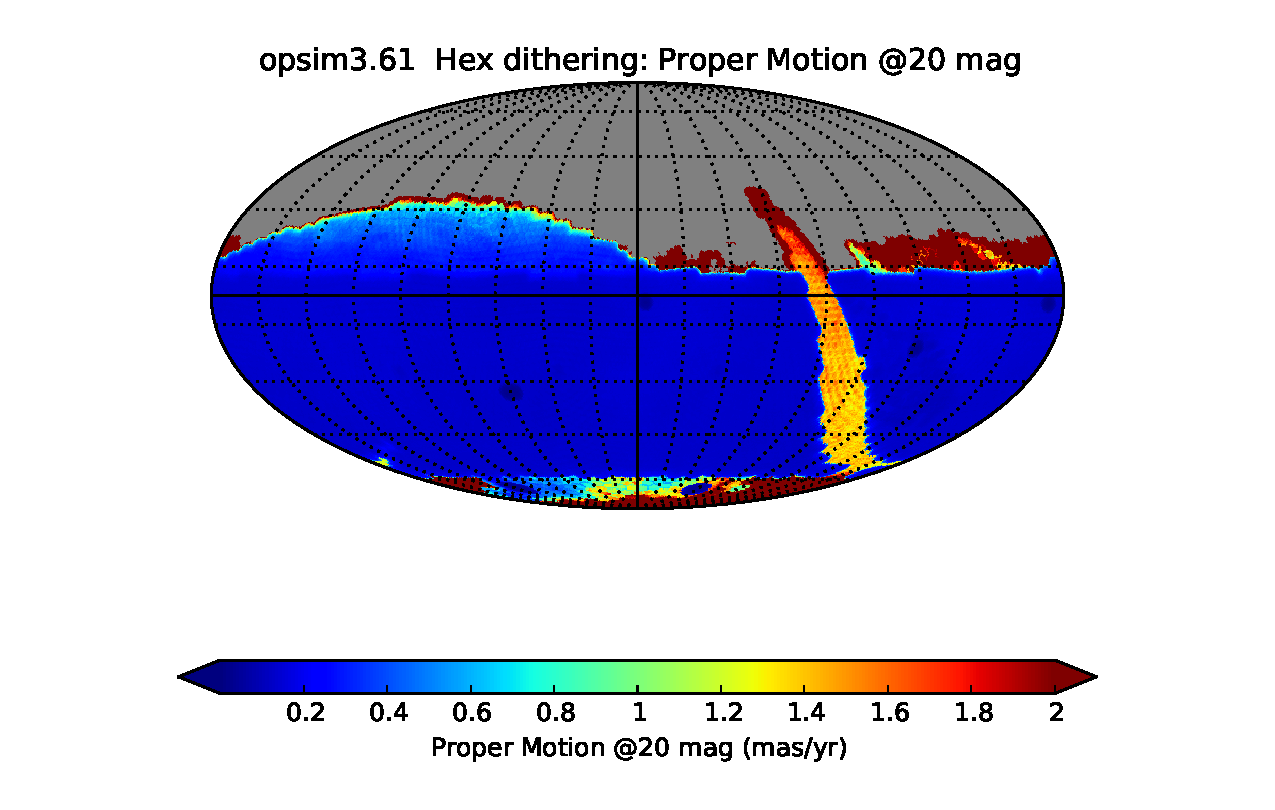
\includegraphics[width=\textwidth]{figures/opsim3_61_Proper_Motion_@20_mag__Hex_dithering_HEAL_SkyMap}
\caption[]{}
\label{subfig:pm20hex}
\end{subfigure}
\begin{subfigure}[]{0.3\textwidth}
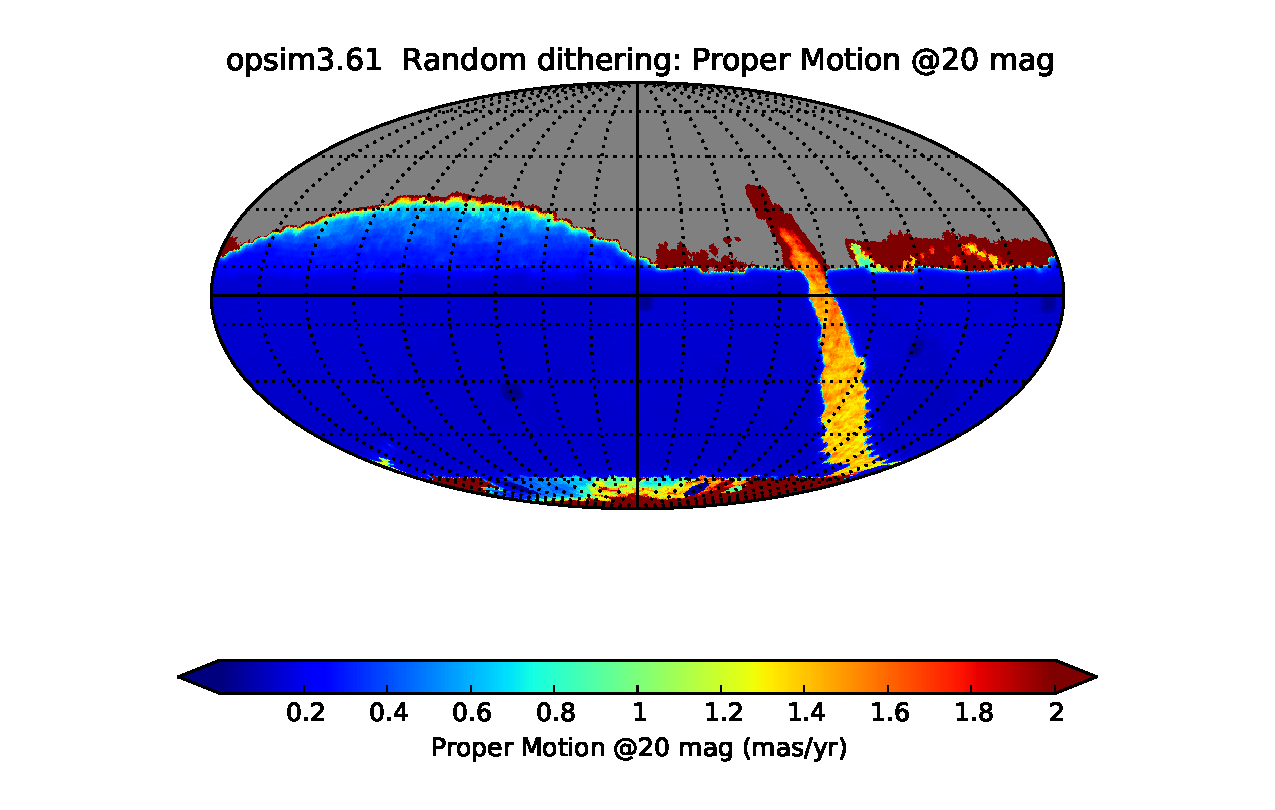
\includegraphics[width=\textwidth]{figures/opsim3_61_Proper_Motion_@20_mag__Random_dithering_HEAL_SkyMap}
\caption[]{}
\label{subfig:pm20random}
\end{subfigure}


\begin{subfigure}[]{0.3\textwidth}
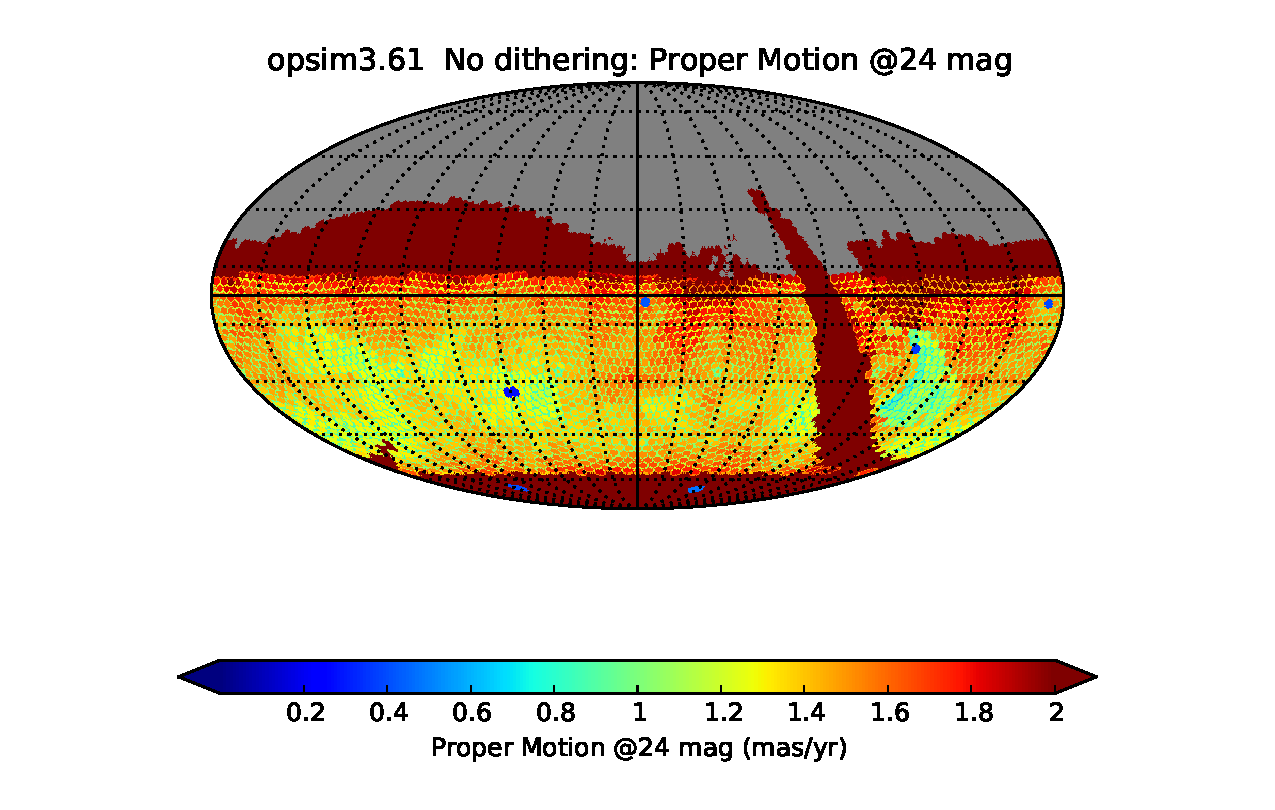
\includegraphics[width=\textwidth]{figures/opsim3_61_Proper_Motion_@24_mag__No_dithering_HEAL_SkyMap}
\caption[]{}
\label{subfig:pm24no}
\end{subfigure}
\begin{subfigure}[]{0.3\textwidth}
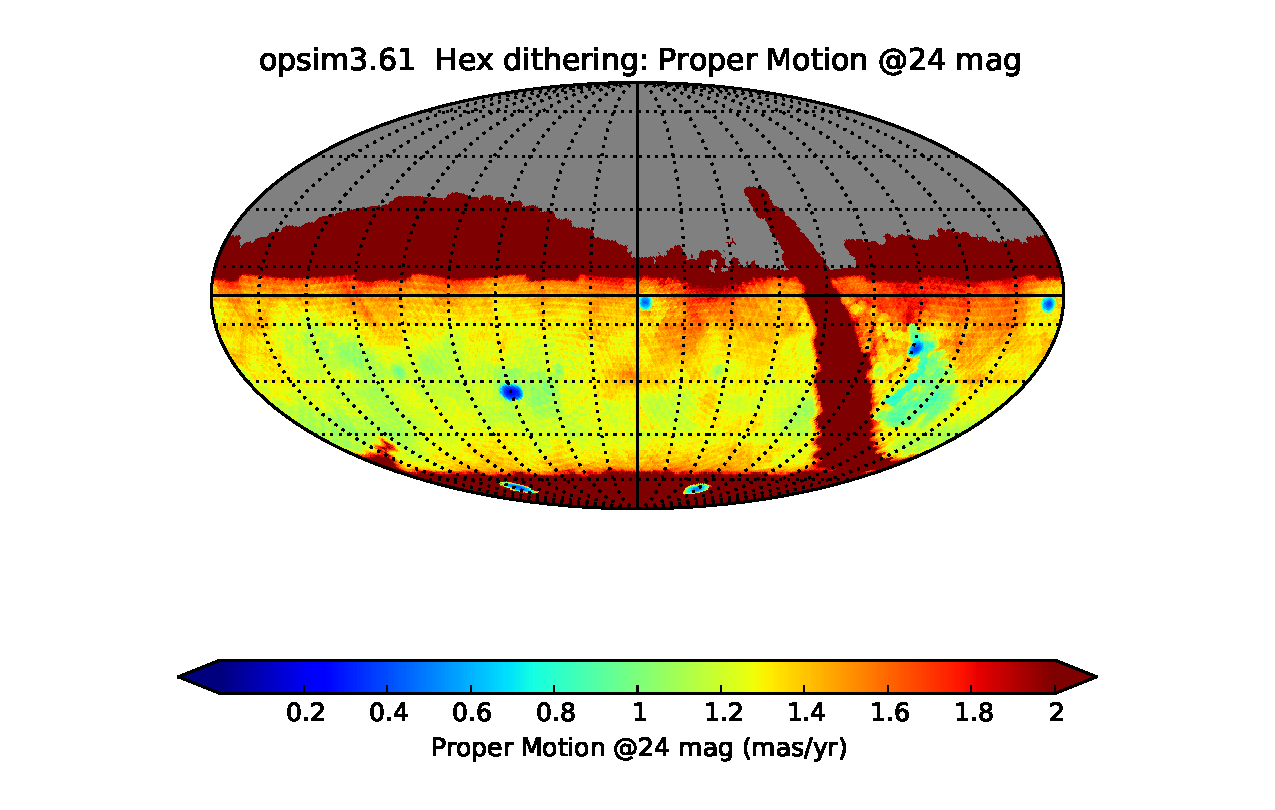
\includegraphics[width=\textwidth]{figures/opsim3_61_Proper_Motion_@24_mag__Hex_dithering_HEAL_SkyMap}
\caption[]{}
\label{subfig:pm24hex}
\end{subfigure}
\begin{subfigure}[]{0.3\textwidth}
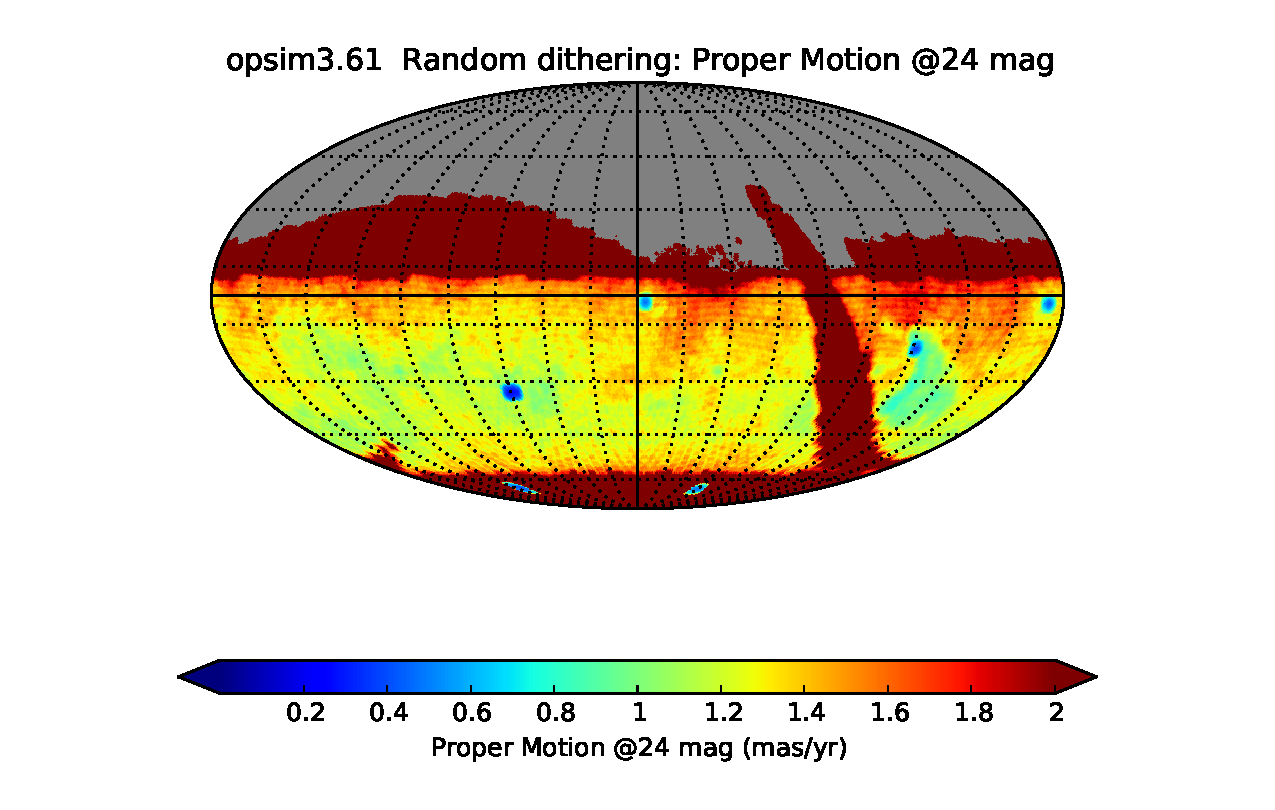
\includegraphics[width=\textwidth]{figures/opsim3_61_Proper_Motion_@24_mag__Random_dithering_HEAL_SkyMap}
\caption[]{}
\label{subfig:pm24random}
\end{subfigure}

\begin{subfigure}[]{0.3\textwidth}
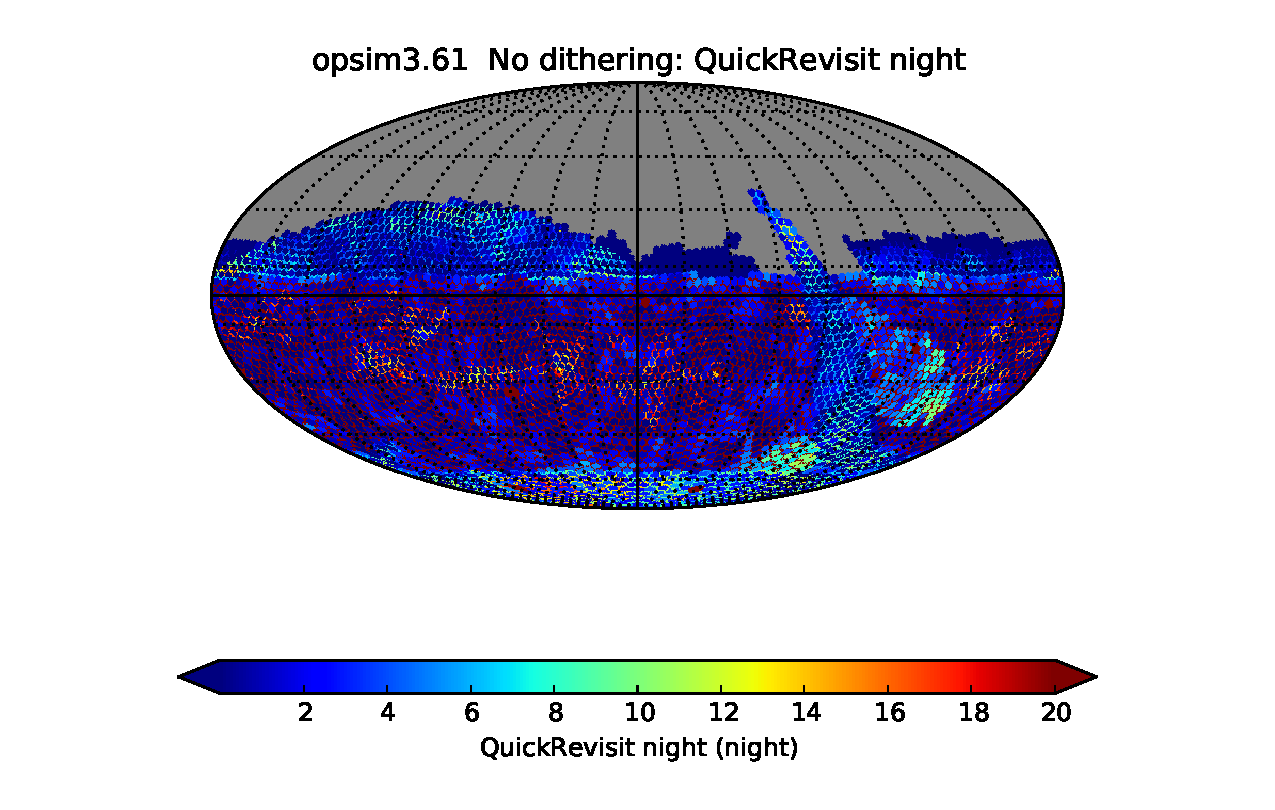
\includegraphics[width=\textwidth]{figures/opsim3_61_QuickRevisit_night__No_dithering_HEAL_SkyMap}
\caption[]{}
\label{subfig:revisitno}
\end{subfigure}
\begin{subfigure}[]{0.3\textwidth}
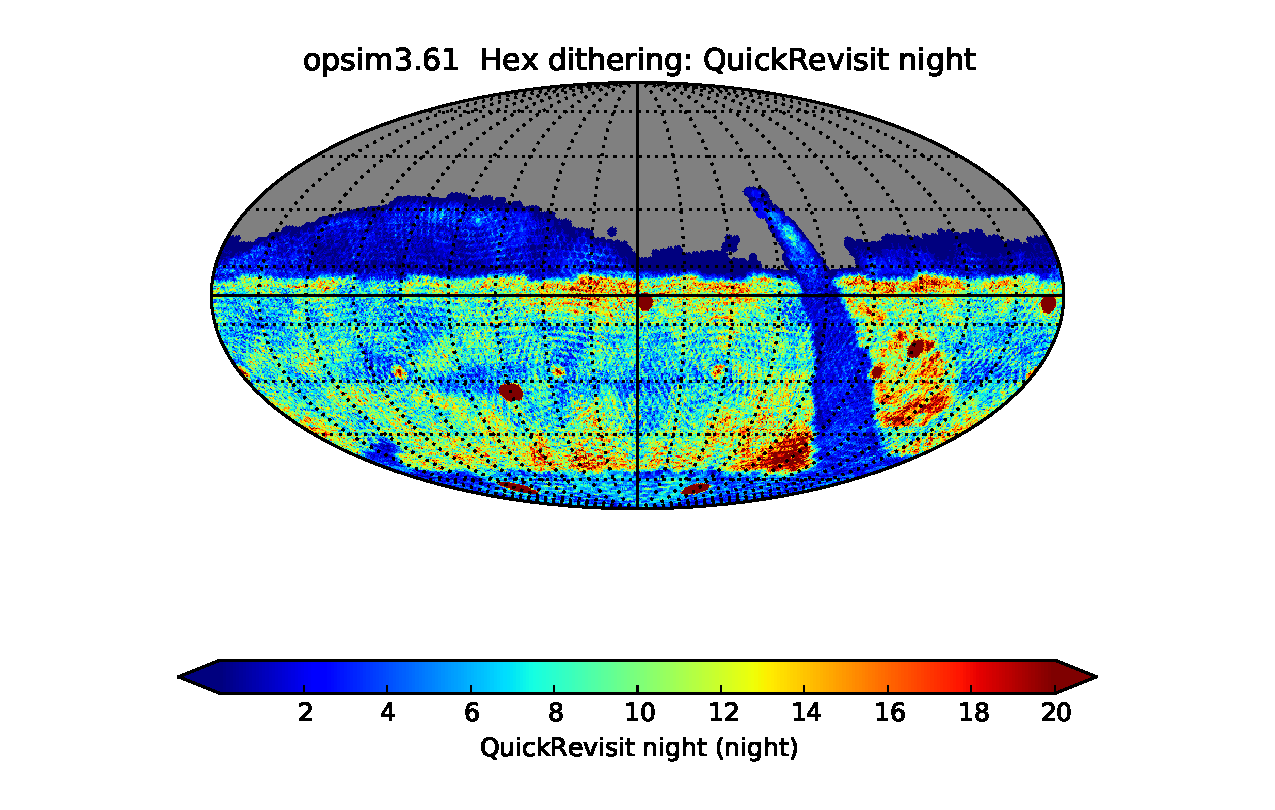
\includegraphics[width=\textwidth]{figures/opsim3_61_QuickRevisit_night__Hex_dithering_HEAL_SkyMap}
\caption[]{}
\label{subfig:revisithex}
\end{subfigure}
\begin{subfigure}[]{0.3\textwidth}
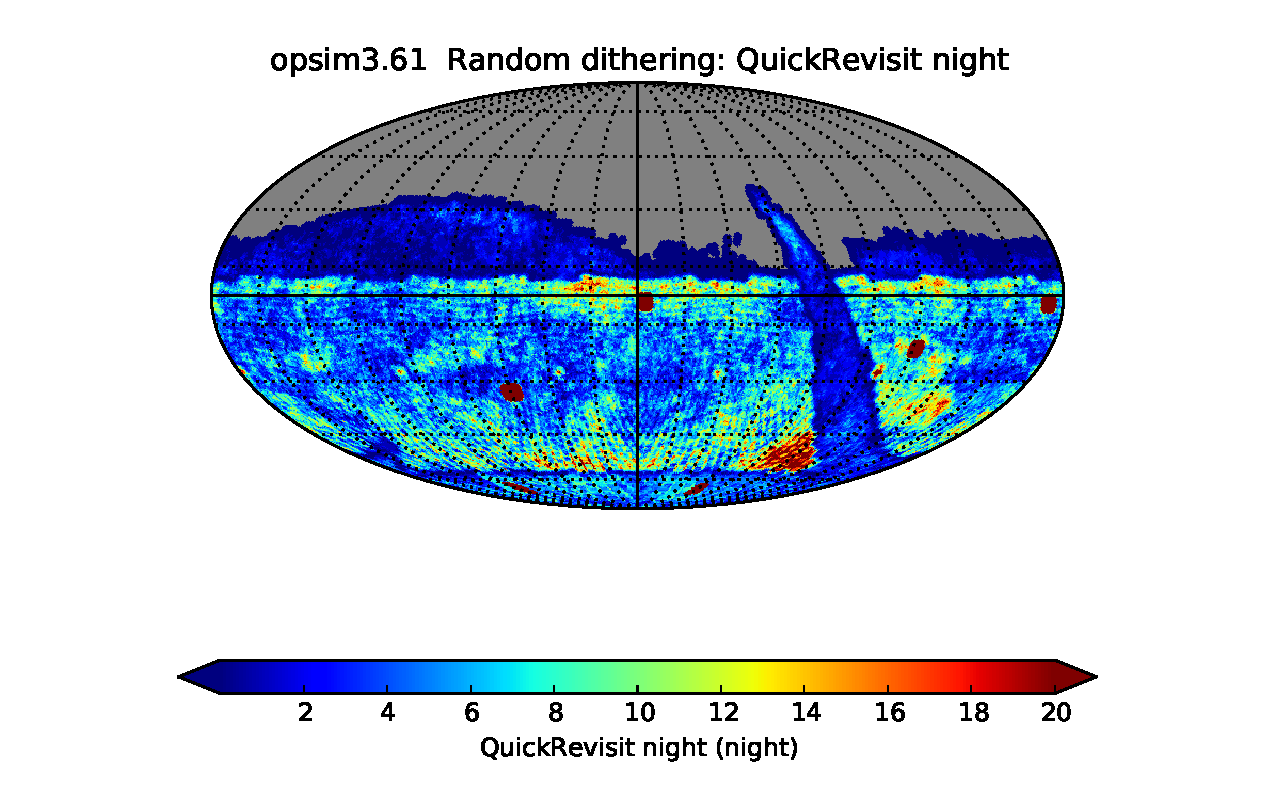
\includegraphics[width=\textwidth]{figures/opsim3_61_QuickRevisit_night__Random_dithering_HEAL_SkyMap}
\caption[]{}
\label{subfig:revisitrandom}
\end{subfigure}

\begin{subfigure}[]{0.3\textwidth}
\centering
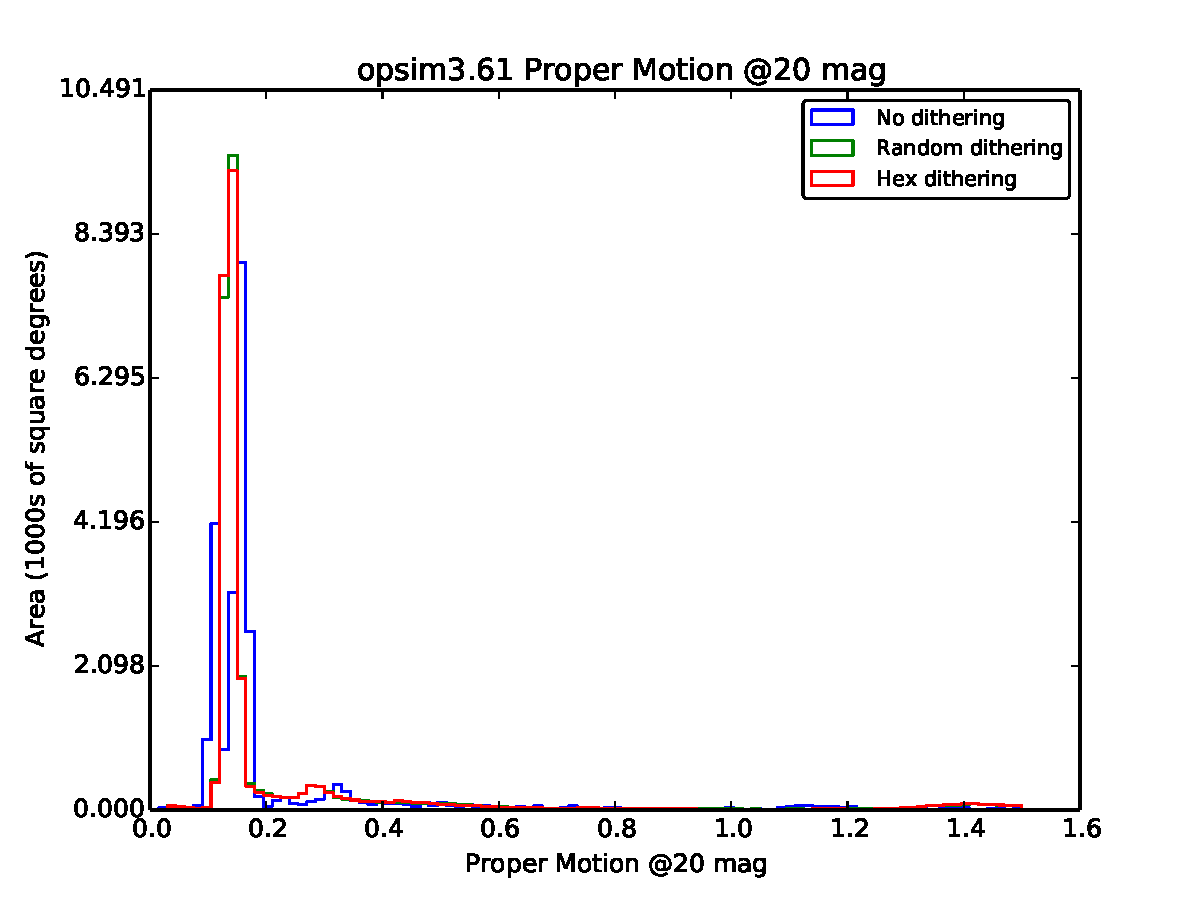
\includegraphics[width=.8\textwidth]{figures/opsim3_61__opsim3_61_Proper_Motion_@20_mag_HEAL_Histogram}
\caption[]{}
\label{subfig:pm20hist}
\end{subfigure}
\begin{subfigure}[]{0.3\textwidth}
\centering
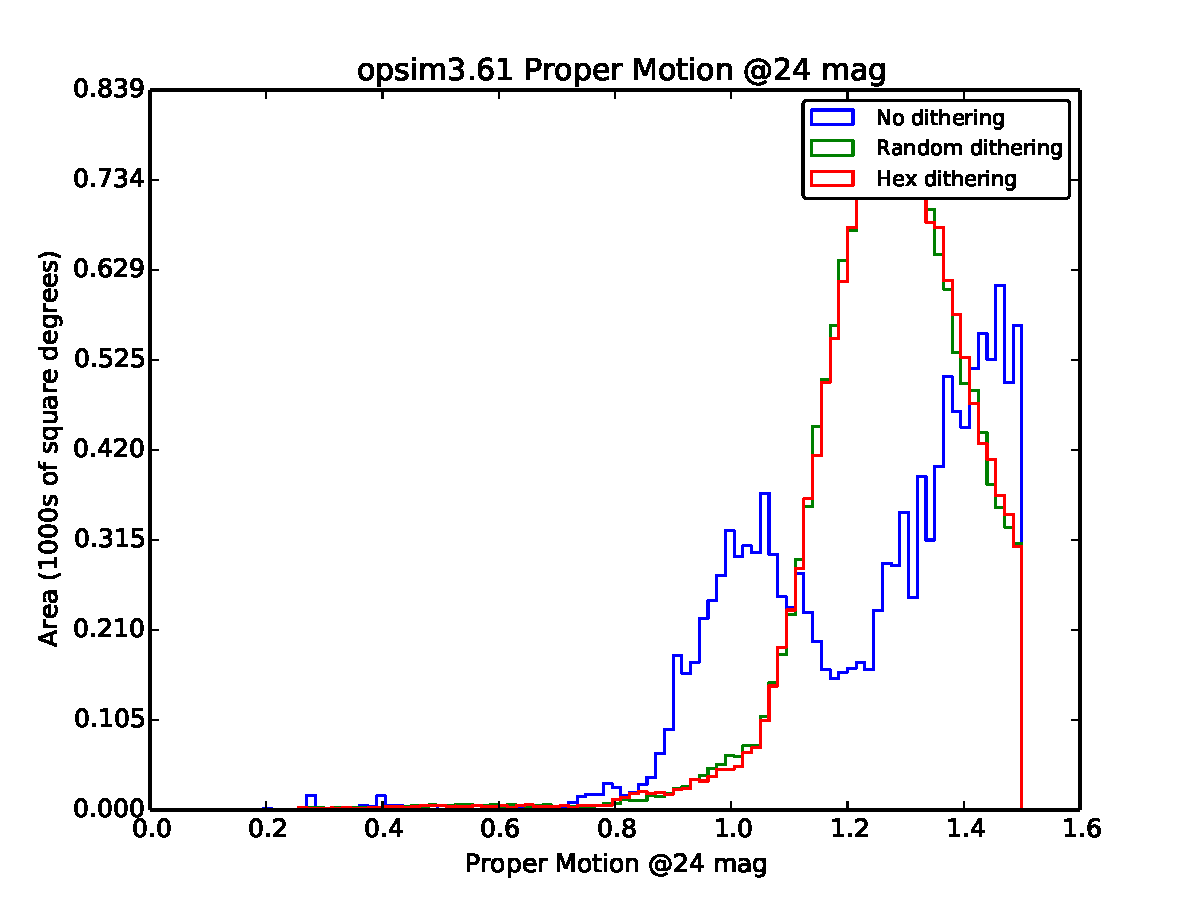
\includegraphics[width=.8\textwidth]{figures/opsim3_61__opsim3_61_Proper_Motion_@24_mag_HEAL_Histogram}
\caption[]{}
\label{subfig:pm24hist}
\end{subfigure}
\begin{subfigure}[]{0.3\textwidth}
\centering
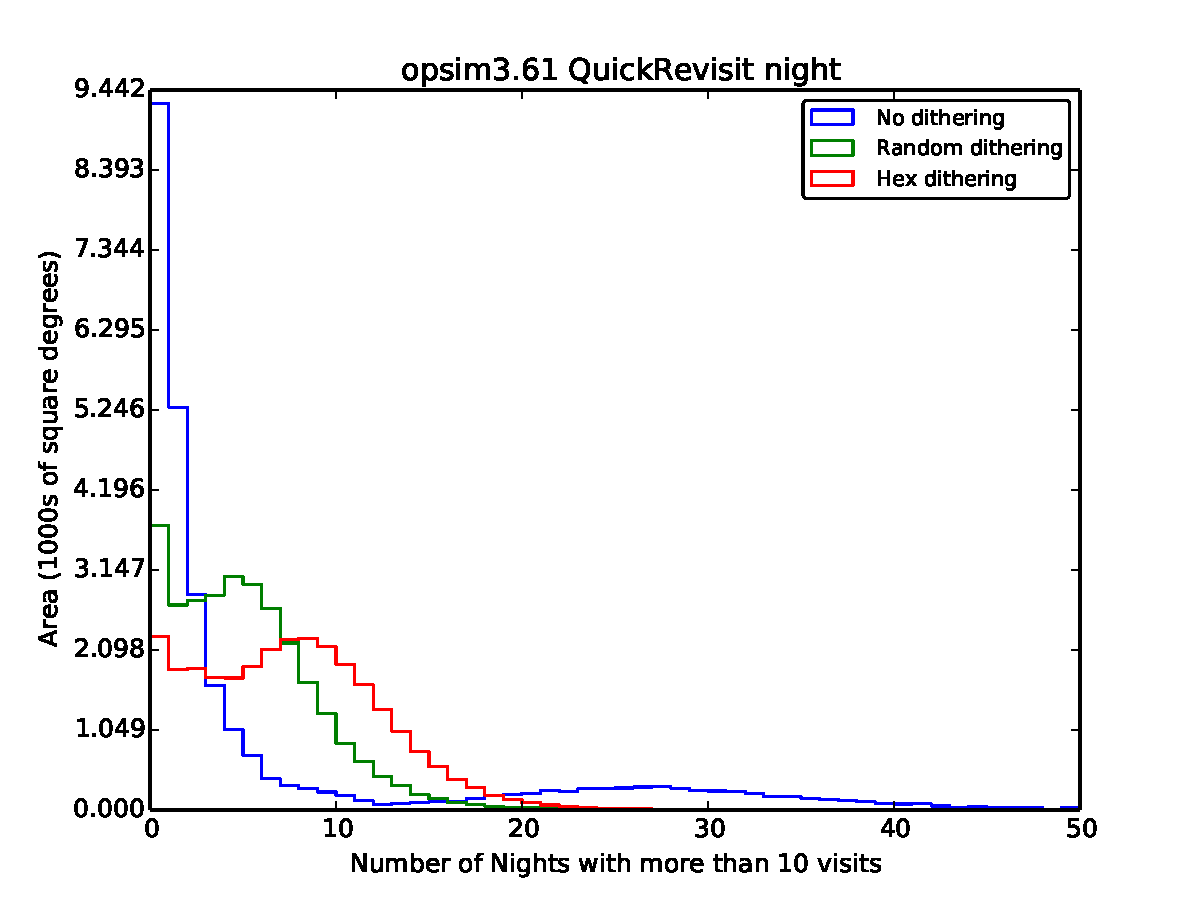
\includegraphics[width=.8\textwidth]{figures/opsim3_61__opsim3_61_QuickRevisit_night_HEAL_Histogram}
\caption[]{}
\label{subfig:revisithist}
\end{subfigure}
\caption[]
{\label{fig:dither_pm_revis}
Analyzing the effects of dithering on proper motion measurements and
the number of nights with more than 10 visits (i.e.,
'QuickRevisits'). Panels~\ref{subfig:pm20no}, \ref{subfig:pm20hex},
and \ref{subfig:pm20random} show the on-sky distribution of expected errors in the
measurement of proper motion for a 20th magnitude star in the case of
no dithering, hex dithering and random dithering, respectively (all visits in
all bands at a particular RA/Dec are used to calculate the proper
motion; the {\tt Metric} assumes there is no parallax to confuse the proper
motion measurement). Panels~\ref{subfig:pm24no}, \ref{subfig:pm24hex},
and \ref{subfig:pm24random} show the same for a 24th magnitude
star. By examining the skymaps and panel~\ref{subfig:pm20hist}, we can
see that dithering is not very important for the proper motion
measurement of high SNR stars, as
generally each measurement is simply running up against the noise
floor of the astrometric measurements (with the notable exception of
the plane of the Milky Way, where fewer visits are obtained). However,
as panel~\ref{subfig:pm24hist} shows, dithering is an important
consideration for lower SNR stars, and improves the median error in
the proper motion by a
about a tenth of a mas/year, presumably due to the increase in the
median number of visits and coadded depth. 
Panels~\ref{subfig:revisitno}, \ref{subfig:revisithex} and
\ref{subfig:revisitrandom} contain plots showing the result of the
{\tt QuickRevisitMetric}, counting the number of nights with more than 10
visits at each RA/Dec grid point. This {\tt Metric} highlights some
differences in the dither strategies, visible in
panel~\ref{subfig:revisithist}. Because the random dither strategy
dithers each visit independently, it can decrease the number of
revisits within a night by spreading these visits over a greater area
and breaking field overlaps. The hex dither preserves relative field
placement within a night, applying a constant offset for the pointings
throughout an entire night. 
}
\end{figure}

By creating {\tt Metrics} tied closely to science goals, we can use MAF to
analyze the effects of different dithering strategies in detail as above. We
can also use MAF to analyze multiple OpSim simulated surveys created
with different simulation parameters such as: varying the exposure time, obtaining visits in
pairs (or singletons or triples), changing the footprint of the
survey, varying the airmass, seeing or skybrightness limits for
obtaining observations, or otherwise changing the cadence goals. This
can be done simply by changing the name of the database in the driver
configuration file (also settable via the command line).  In
this way, MAF can be used to evaluate different observing strategies. 

\begin{table}[]
\caption{Summary statistics of {\tt Metrics} applied to non-dithered,
  hex dithered, and randomly dithered OpSim pointings using a {\tt
    HealpixSlicer} with resolution of 27.4\arcsec.}
\label{tab:summarystats}
\begin{center}
\begin{tabular}{|l|l|l|l|l|}
\hline
MetricName &  Metadata &  Median &  Mean &  RobustRMS \\
\hline  
\hline 
Nvisits g band (\#)&  g No dithering & 79.00 & 93.80 & 20.76\\  
Nvisits g band (\#) &  g Hex dithering & 98.00 & 92.17 & 31.13\\ 
Nvisits g band (\#)&  g Random dithering & 98.00 & 91.68 & 33.36\\ 
Nvisits r band (\#)&  r No dithering & 174.00 & 195.00 & 60.04\\  
Nvisits r band (\#) &  r Hex dithering & 217.00 & 192.72 & 94.89\\ 
Nvisits r band (\#)&  r Random dithering & 217.00 & 190.99 & 103.04\\ 
\hline
Coadded m5 g band (mag) &  g No dithering & 27.13 & 26.98 & 0.21\\ 
Coadded m5 g band (mag)&  g Hex dithering & 27.24 & 26.99 & 0.28\\
Coadded m5 g band (mag)&  g Random dithering & 27.23 & 26.99 & 0.30\\
Coadded m5 r band (mag)&  r No dithering & 27.34 & 27.04 & 0.28\\ 
Coadded m5 r band (mag)&  r Hex dithering & 27.45 & 27.07 & 0.43\\
Coadded m5 r band (mag)&  r Random dithering & 27.45 & 27.06 & 0.49\\
\hline
Proper Motion @20 mag  (mas yr$^{-1}$)&   No dithering & 0.16 & - & 0.12\\ 
Proper Motion @20 mag  (mas yr$^{-1}$)&   Hex dithering & 0.14 & - & 0.11\\
Proper Motion @20 mag  (mas yr$^{-1}$)&   Random dithering & 0.14 & - & 0.11\\
Proper Motion @24 mag  (mas yr$^{-1}$)&   No dithering & 1.54 & - & 2.73\\ 
Proper Motion @24 mag  (mas yr$^{-1}$)&   Hex dithering & 1.42 & - & 2.23\\
Proper Motion @24 mag  (mas yr$^{-1}$)&   Random dithering & 1.42 & - & 2.23\\
\hline
QuickRevisit night (\# nights)&   No dithering & 1.00 & 7.84 & 5.19\\ 
QuickRevisit night (\# nights)&   Hex dithering & 7.00 & 7.70 & 5.19\\
QuickRevisit night (\# nights)&   Random dithering & 4.00 & 6.35 & 3.71\\
\hline
\end{tabular}
\end{center}
\end{table}

%% < ResultsSummary.dat grep Mean | sed 's/Mean://g' | sed 's/Median://g' | sed 's/RobustRms://g' | awk -F',' 'BEGIN {OFS=" & "; ORS="\\\\\n"} {$14=sprintf("%.2f", $14); $15=sprintf("%.2f", $15); $16=sprintf("%.2f", $16)} {print $1, $4, $15, $16, $14}'

\section{Writing a new {\tt Metric}}
\label{sec:MetricAPI}

We anticipate that many users will want to write their own {\tt Metrics}.
The {\tt Metric} class API is minimal to help accommodate
this. A base class provides the framework overhead, such as creating a
column registry (so that the framework can determine what columns to
fetch from the database) and determining units for each column if not
provided by the user (so that plots can be properly labeled). This
leaves the user free to concentrate on the code relevant to their
particular analysis.

Each {\tt Metric} must have {\it \_\_init\_\_} and {\it run} methods. The
{\it run} method is given only the data slice and the slicePoint
metadata{\footnote{Many {\tt Metrics} will not use the slicePoint
    metadata, but since the {\tt Driver} uses 
    {\tt Metrics} interchangeably, the arguments passed to the {\it
      run} method are the same for all {\tt Metrics}.}, applies the algorithm
to calculate the metric value, and returns only that metric value for
that data slice. For the simplest metrics,
operating on a single column and returning a scalar value for each
data slice, the user only needs to write the {\it run} method.  An
example of a simple {\tt Metric}, providing only a new {\it run} method is
shown in Figure~\ref{fig:simplemetric}. Simple Metrics like these
inherit from {\tt SimpleScalarMetric}, which is a subclass of the {\tt BaseMetric}
that provides some additional error checking about column names and
returned data types.

\begin{figure}
\centering
\begin{lstlisting}[frame=single]
class RobustRmsMetric(SimpleScalarMetric):
    """
    Use the inter-quartile range of the data to estimate the RMS.  
    Robust since this calculation does not include outliers in the
    distribution.
    """
    def run(self, dataSlice, slicePoint):
        iqr = np.percentile(dataSlice[self.colname], 75) - 
             np.percentile(dataSlice[self.colname], 25)
        rms = iqr/1.349 #approximation
        return rms
\end{lstlisting}
\caption[]
{ \label{fig:simplemetric} Example of writing a new simple {\tt Metric},
  operating on a single data column and returning a scalar value for
  each data slice. The class inherits from {\tt SimpleScalarMetric} and uses
  this {\it \_\_init\_\_} method, but provides its own {\it run}
  method. }
\end{figure}

By also extending the {\tt SimpleScalarMetric}'s {\it \_\_init\_\_} method using Python's {\it super}, users can provide
configurable parameters to each metric at run time or add their own
column definitions. An example is the {\tt PercentileMetric} shown in
Figure~\ref{fig:simpleconfigurablemetric}. 

\begin{figure}
\begin{lstlisting}[frame=single]
class PercentileMetric(SimpleScalarMetric):
    def __init__(self, colname, percentile=90, **kwargs):
        super(PercentileMetric, self).__init__(colname, **kwargs)
        self.percentile = percentile
    def run(self, dataSlice, slicePoint):
        return np.percentile(dataSlice[self.colname], self.percentile)
\end{lstlisting}
\caption[]
{\label{fig:simpleconfigurablemetric} Example of writing a new simple
  {\tt Metric} that includes a run-time configurable parameter (the
  percentile value). The class inherits from the {\tt SimpleScalarMetric},
  but extends the {\it \_\_init\_\_} method, while still providing its
  own {\it run} method.}
\end{figure}

More complicated {\tt Metrics}, such as those operating on more than one
column or returning a complex data type (such as a dictionary or an
array), inherit directly from the {\tt BaseMetric}. In addition, those
returning a complex data type can add `reduce' methods, intended to
take that complex data value and turn it into a scalar for each
slice. This is especially useful for {\tt Metrics} where a computationally
expensive value must be computed but then could be interpreted in
multiple ways to produce scalar values at each slicePoint for
visualization.  First the {\tt Metric} {\it run} is called for each data
slice; then all {\it reduce} methods are called for each data slice
(but passed the metric value calculated by the {\it run} method at
that point).

An example is the {\tt VisitGroupsMetric}:
this {\tt Metric} is intended to examine how visits are paired together as a
preliminary exploration of how well an OpSim simulated survey might perform for solar
system object discovery. First the {\tt Metric} calculates the number of visits
within a given time interval on each night, for each data slice,
returning a dictionary containing the nights that multiple visits were
achieved and the total number of visits on each of those nights that
were within the time interval. Then different {\it reduce} methods
operate on each metric value (corresponding to each original data slice),
calculating the median number of visits, the number of times that more
than a threshold number of visits occurred within some larger time
interval of number of nights, the number of lunations that received
more than a threshold number of nights with multiple visits, and
the number of successive lunations that received more than a
threshold number of nights with multiple visits. The reduce methods
provide multiple views into the underlying question (how visits are
paired together for discovering solar system objects) and are all
desirable; however, the first step is somewhat computationally
expensive. By allowing multiple reduce methods, we can take the
original data slice and end up examining it in multiple ways with
minimal cost. Code for the {\tt VisitGroupsMetric} can be found online in
the LSST Stash repository at {\url {http://ls.st/rkw}},
but excerpts illustrating the {\it run} and {\it reduce}
methods are shown in Figure~\ref{fig:visitgroups}. 

\begin{figure}
\begin{lstlisting}[frame=single]
class VisitGroupsMetric(BaseMetric):
    """Count the number of visits per night within deltaTmin and deltaTmax."""
    def __init__(self, timesCol='expMJD', nightsCol='night', 
                 deltaTmin=15.0/60.0/24.0, deltaTmax=90.0/60.0/24.0, minNVisits=2, window=30, minNNights=3,
                 **kwargs):
  #... <snip> ... # Removed lines setting internal variables to passed values
        super(VisitGroupsMetric, self).__init__([self.times, self.nights], **kwargs)

    def run(self, dataSlice):
        """
        Return a dictionary of:
         the number of visits within a night (within delta tmin/tmax of another visit),
         and the nights with visits > minNVisits.
        Count two visits which are within tmin of each other, but which have another visit
         within tmin/tmax interval, as one and a half (instead of two).
        """
        uniquenights = np.unique(dataSlice[self.nights])
        nights = []
        visitNum = []
  #... <snip> ... # Removed lines with details of calculation
        metricval = {'visits':visitNum, 'nights':nights}
        if len(visitNum) == 0:
            return self.badval
        return metricval
        
    def reduceMedian(self, metricval):
        """Reduce to median number of visits per night (2 visits = 1 pair)."""
        return np.median(metricval['visits'])
        
    def reduceNNightsWithNVisits(self, metricval):
        """Reduce to total number of nights with more than 'minNVisits' visits."""
        condition = (metricval['visits'] >= self.minNVisits)
        return len(metricval['visits'][condition])

    def reduceNVisitsInWindow(self, metricval):
        """Reduce to max number of total visits on all nights with more than minNVisits, within any 'window' (default=30 nights)."""
        maxnvisits = 0
        for n in metricval['nights']:
            vw, nw = self._inWindow(metricval['visits'], metricval['nights'], n, self.window, self.minNVisits)
            maxnvisits = max((vw.sum(), maxnvisits))
        return maxnvisits
\end{lstlisting}
\caption[]
{\label{fig:visitgroups} Example of a more complex {\tt Metric} that returns
a dictionary from the {\it run} method and then provides several {\it
  reduce} methods to evaluate different aspects of those calculated
values. Both the {\it run} method and the {\it reduce} methods are
called for each slice in the {\tt Slicer}.}
\end{figure}

More information on writing and using your own {\tt Metrics} is available in
the MAF documentation. 


\section{Conclusions}

MAF has been designed to provide an easy to use, easy to extend
framework to analyze LSST OpSim simulated surveys. It is a powerful
tool for evaluating the effects of observing strategies, including
dithering strategies.  By collaborating with the wider LSST community
to create new {\tt Metrics} covering a wide range of science cases, we hope
to discover optimal strategies for the scheduling of LSST and quantify
both the overall efficiency of the surveys and their scientific
potential.

Beyond analyzing LSST OpSim outputs, MAF can be applied to any
dataset. Much of the necessary framework requirements are available in
base classes (as well as an illustration of the required API), which
can be extended for use with a particular dataset. For example, if a
user writes a custom {\tt Metric} and uses that with one of MAF's
{\tt Slicers} (or writes their own {\tt Slicer} for a specific purpose), but then
wants to analyze observing histories from other telescopes instead of
(or as well as) LSST OpSim data, all that is required is a new
{\tt Database} class to access the new pointing history.

We intend to continue development on MAF, in particular improving the
presentation of MAF outputs using a web interface. In addition, we
welcome community contributions to MAF, including new {\tt Metrics},
{\tt Slicers}, or {\tt Database} classes. There are several avenues
for input including direct contact with the LSST
Simulations group ({\url{lsst-imsim@lsstcorp.org}}),
 a series of workshops on the OpSim observing
strategy, to be hosted by NOAO and LSST, starting August 2014 with the
`LSST Observing Cadences Workshop' ({\url{http://ls.st/2xd}}), 
and we will be hosting contributed code within the LSST Stash
repository. 

\appendix
\section{URLs}
\label{app:urls}

This section contains the expansion of the shortened URLs in the body
of this paper, along with a brief summary of the content at the URL
location. All URLs are current at the time of this paper's
publication.

MAF documentation is hosted at:
{\url {http://ls.st/ziz}}
 (expands to 
{\url {https://confluence.lsstcorp.org/display/SIM/MAF+documentation}}).

The MAF git repository is hosted at:
{\url {http://ls.st/pxj}}
(expands to 
{\url {https://stash.lsstcorp.org/projects/SIM/repos/sims_maf/}}).

The full example MAF driver script is available at: 
{\url {http://ls.st/mxl}}
 (expands to 
{\url
  {https://stash.lsstcorp.org/projects/SIM/repos/sims_maf/browse/doc/SPIE_2014/testdriver2.py?at=refs\%2Fheads\%2Ffeature\%2FOPSIM-461-spie-paper-for-maf}}}).

The {\tt VisitGroupsMetric} class can be browsed in the LSST Stash
repository at:
{\url {http://ls.st/rkw}}
 (expands to
{\url
  {https://stash.lsstcorp.org/projects/SIM/repos/sims_maf/browse/python/lsst/sims/maf/metrics/visitGroupsMetric.py}}). 

Details about the first joint NOAO and LSST Observing Cadences
Workshop are available at:
{\url {http://ls.st/2xd}}
(expands to 
{\url {https://project.lsst.org/meetings/ocw/}}). 


%%%%%%%%%%%%%%%%%%%%%%%%%%%%%%%%%%%%%%%%%%%%%%%%%%%%%%%%%%%%%
\acknowledgments     %>>>> equivalent to \section*{ACKNOWLEDGMENTS}       

We would like to thank Alex Kim, Seth Digel, Phil Marshall, Knut Olsen, and Michael Woods-Vasey for participating in beta testing and providing feedback on early documentation for MAF. 

LSST project activities are supported in part by the National Science Foundation through Cooperative Support Agreement (CSA) Award No. AST-1227061 under Governing Cooperative Agreement 1258333 managed by the Association of Universities for Research in Astronomy (AURA), and the Department of Energy under contract with the SLAC National Accelerator Laboratory.   Additional LSST funding comes from private donations, grants to universities, and in-kind support from LSSTC Institutional Members.


%%%%%%%%%%%%%%%%%%%%%%%%%%%%%%%%%%%%%%%%%%%%%%%%%%%%%%%%%%%%%
%%%%% References %%%%%

\bibliography{spie_ref}   %>>>> bibliography data in report.bib
\bibliographystyle{spiebib}   %>>>> makes bibtex use spiebib.bst

\end{document}

%%  LocalWords:  showstringspaces formfeed newpage tabsize basicstyle
%%  LocalWords:  commentstyle breaklines MAF OpSim downtime metadata
%%  LocalWords:  APIs API numpy RA HealpixSlicer Healpixel MeanMetric
%%  LocalWords:  RobustRMS FullRange HealPixel FieldID OpSimFieldID
%%  LocalWords:  UniSlicer OneDSlicer Diaconis numpy's NDSlicer kd zp
%%  LocalWords:  OpSimFieldSlicer FieldIDs Healpix Healpixels HEALpix
%%  LocalWords:  tesselation slicePoint slicePoints SliceMetric MAF's
%%  LocalWords:  recarray SQLAlchemy OpsimDatabase sqlite IDs Opsim
%%  LocalWords:  Stackers sliceMetric dataSlice RmsMetric params 
%%  LocalWords:  IdentityMetric summaryStats makeMetricConfig sql col
%%  LocalWords:  makeSlicerConfig metricDict makeDict configList ONED
%%  LocalWords:  CountMetric OneDSlicers kwargs metricName histMerge
%%  LocalWords:  histNum legendloc xlabel sliceColName coadded NSIDE
%%  LocalWords:  pointings Coaddm healpixel SkyMap healpy's anafast
%%  LocalWords:  PowerSpectrum skymap mags zeropoint plotDict mag Co
%%  LocalWords:  zpoint fieldRA fieldDec hexdither hexdithra utils np
%%  LocalWords:  hexdithdec hexdithered addCols spatialkey config def
%%  LocalWords:  coadd RandomDither maxDither init raCol decCol rad
%%  LocalWords:  randomSeed colsAdded randomRADither randomDecDither
%%  LocalWords:  colsReq simData dithersRA len dithersDec cos dec XXX
%%  LocalWords:  ProperMotionMetric QuickRevisitMetric astrometric vw
%%  LocalWords:  SNR revis QuickRevisit QuickRevisits skymaps mas csv
%%  LocalWords:  dithers skybrightness MetricName ResultsSummary grep
%%  LocalWords:  sed awk OFS ORS SimpleScalarMetric BaseMetric args
%%  LocalWords:  RobustRmsMetric iqr colname SimpleScalarMetric's nw
%%  LocalWords:  Python's PercentileMetric VisitGroupsMetric timesCol
%%  LocalWords:  lunations deltaTmin deltaTmax expMJD nightsCol tmin
%%  LocalWords:  minNVisits minNNights tmax uniquenights visitNum CSA
%%  LocalWords:  metricval badval reduceMedian reduceNVisitsInWindow
%%  LocalWords:  reduceNNightsWithNVisits maxnvisits inWindow nVisits
%%  LocalWords:  makeBinnerConfig outputDir dbAddress opsimName nside
%%  LocalWords:  plotRange scaleStretchDesign zpoints coaddedDepth
%%  LocalWords:  nvisits dithlabels slicerNames HealpixSlicerRandom
%%  LocalWords:  HealpixSlicerDither dithlabel slicerName elif rmag
%%  LocalWords:  slicerkwargs slicermetadata nVisitsInNight plotMin
%%  LocalWords:  plotMax histMin histMax MedianMetric seeingCol Vasey
%%  LocalWords:  percentileClip cbarFormat healpix AST SLAC LSSTC ref
%%  LocalWords:  spie bibtex spiebib bst
